
The performance of track and TAS based tagging variables with the default angular weighting of $\beta=1$ is compared to the corresponding calorimeter variables for $W$ boson, Higgs boson and Top quark identification. 
The stated signal efficiencies are calculated after the mass cut plus tagging with n-Subjettiness or C2/D2. Therefore, the endpoint of the ROCs is at 68\% signal efficiency, the fraction kept after the mass cut. Consequently, it is required to achieve a tagging only signal efficiency of $\frac{0.5}{0.68} \sim 0.74$ for a signal efficiency of 0.5 after mass cut and tagging. Similarly, the stated and compared background rejections result from the multiplication of both, thus representing the QCD rejection of the combined mass- and tagging variable-cut. 
The complete set of signal and background distributions for different inputs can be found in the Appendix \ref{app:sascha}.

\subsubsection{Performance for $W$ boson tagging}
Shown in Figure \ref{fig:w_distribution_example} are exemplary signal and background distributions in intermediate $p_T$ bins compared for different inputs. This shows throughout narrower signal distributions rising slightly sharper for tracks and assisted tracks compared to calorimeter clusters which can be explained by the high angular resolution. The right handed tails of the signal distributions are similar to the calorimeter variables. Similarly, the background distributions shift as well, but not as distinct as seen for the signal.
\begin{figure}[htp]
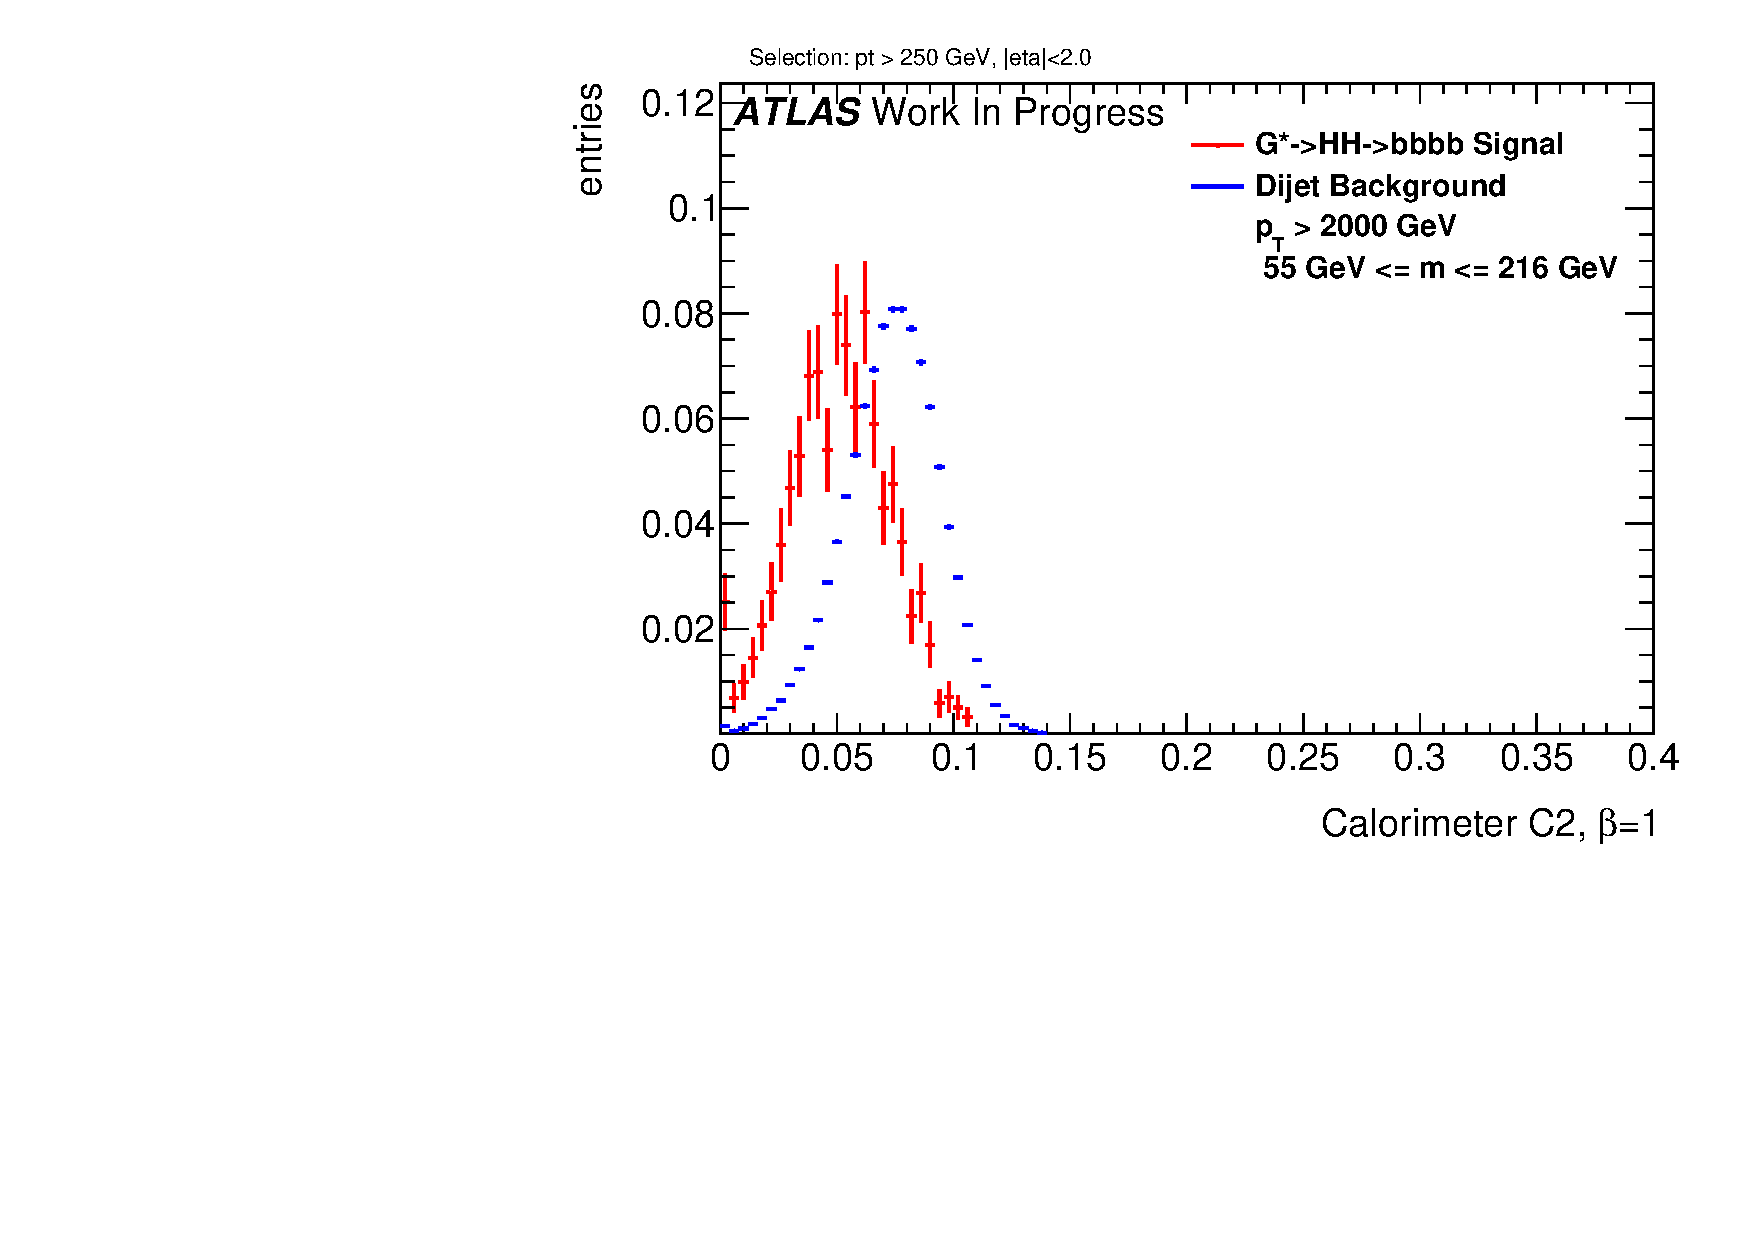
\includegraphics[width=0.3\textwidth]{sascha_input/plots/W/Beta1/h_recoJet_C2_bin6.pdf} 
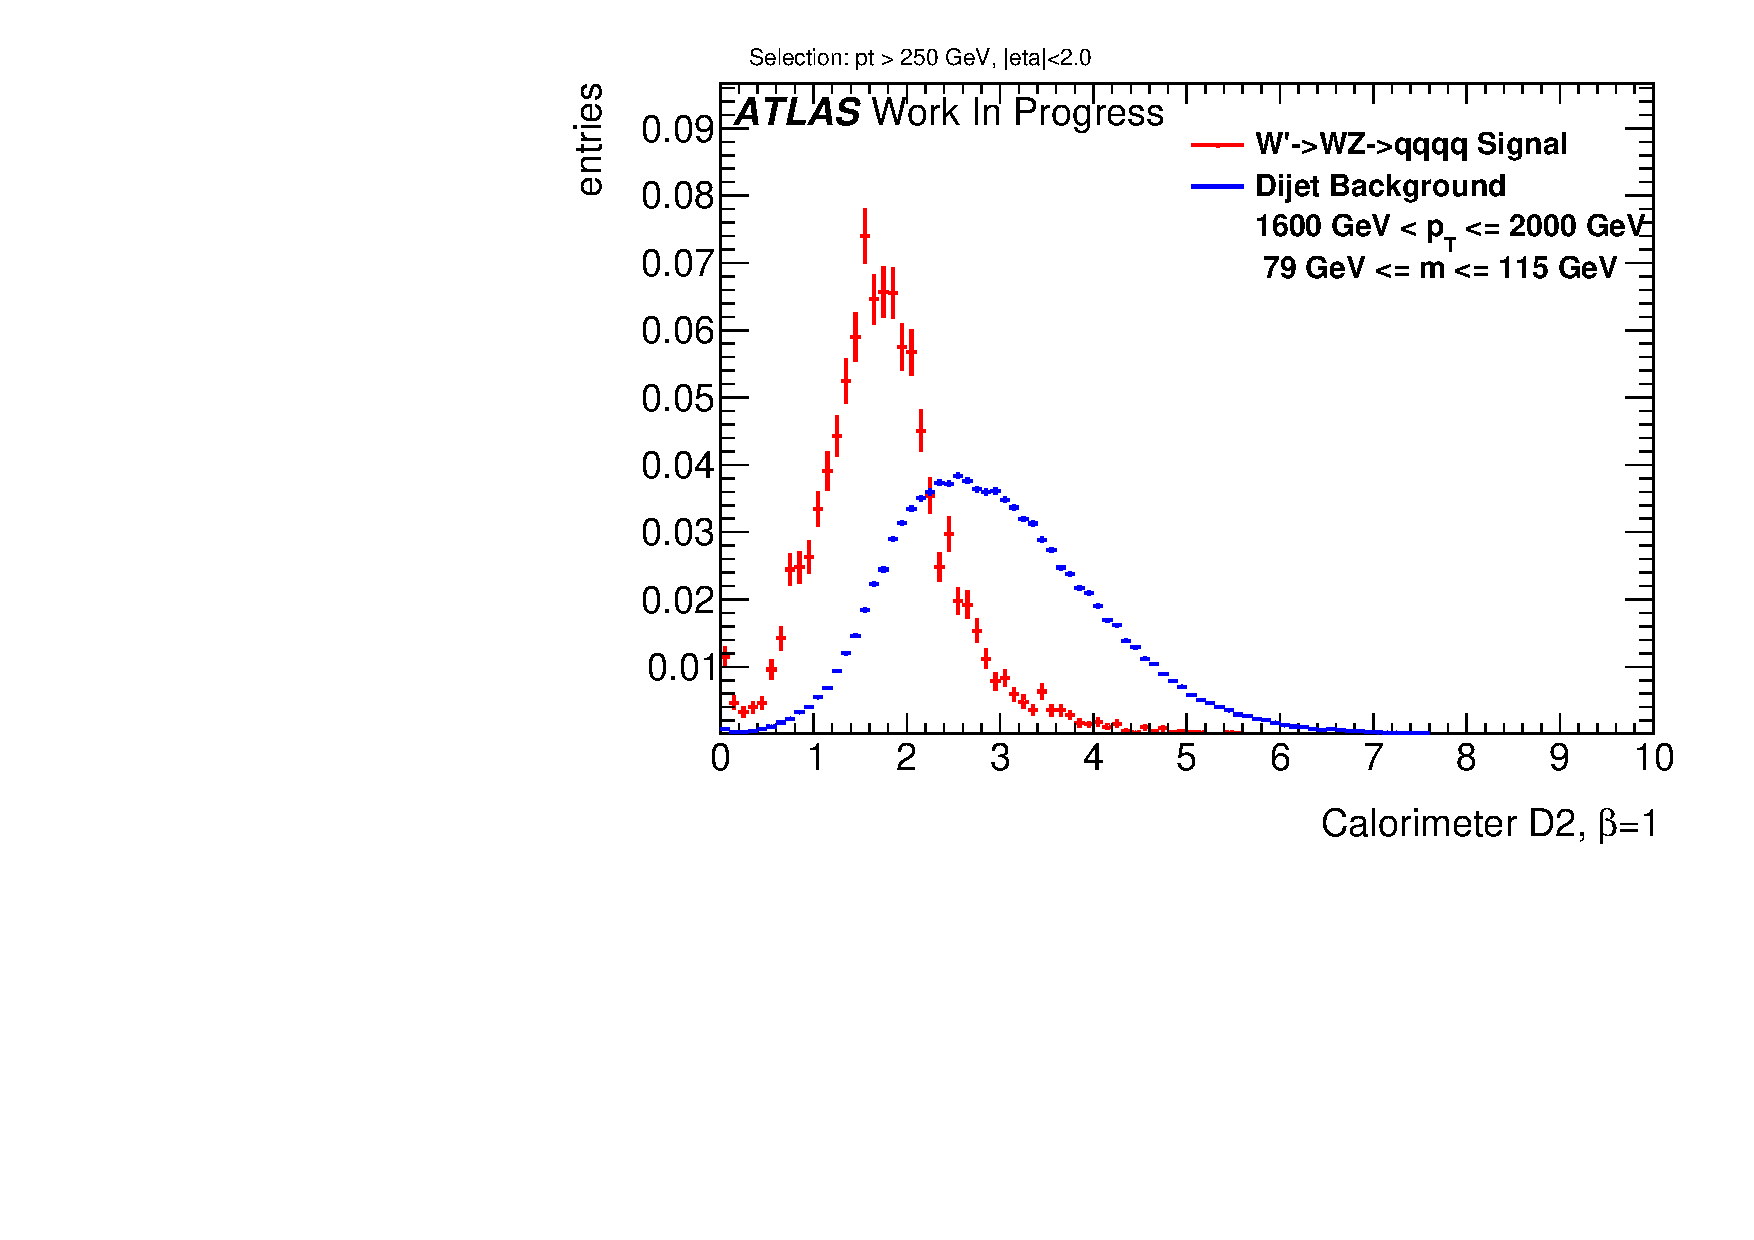
\includegraphics[width=0.3\textwidth]{sascha_input/plots/W/Beta1/h_recoJet_D2_bin5.pdf} 	
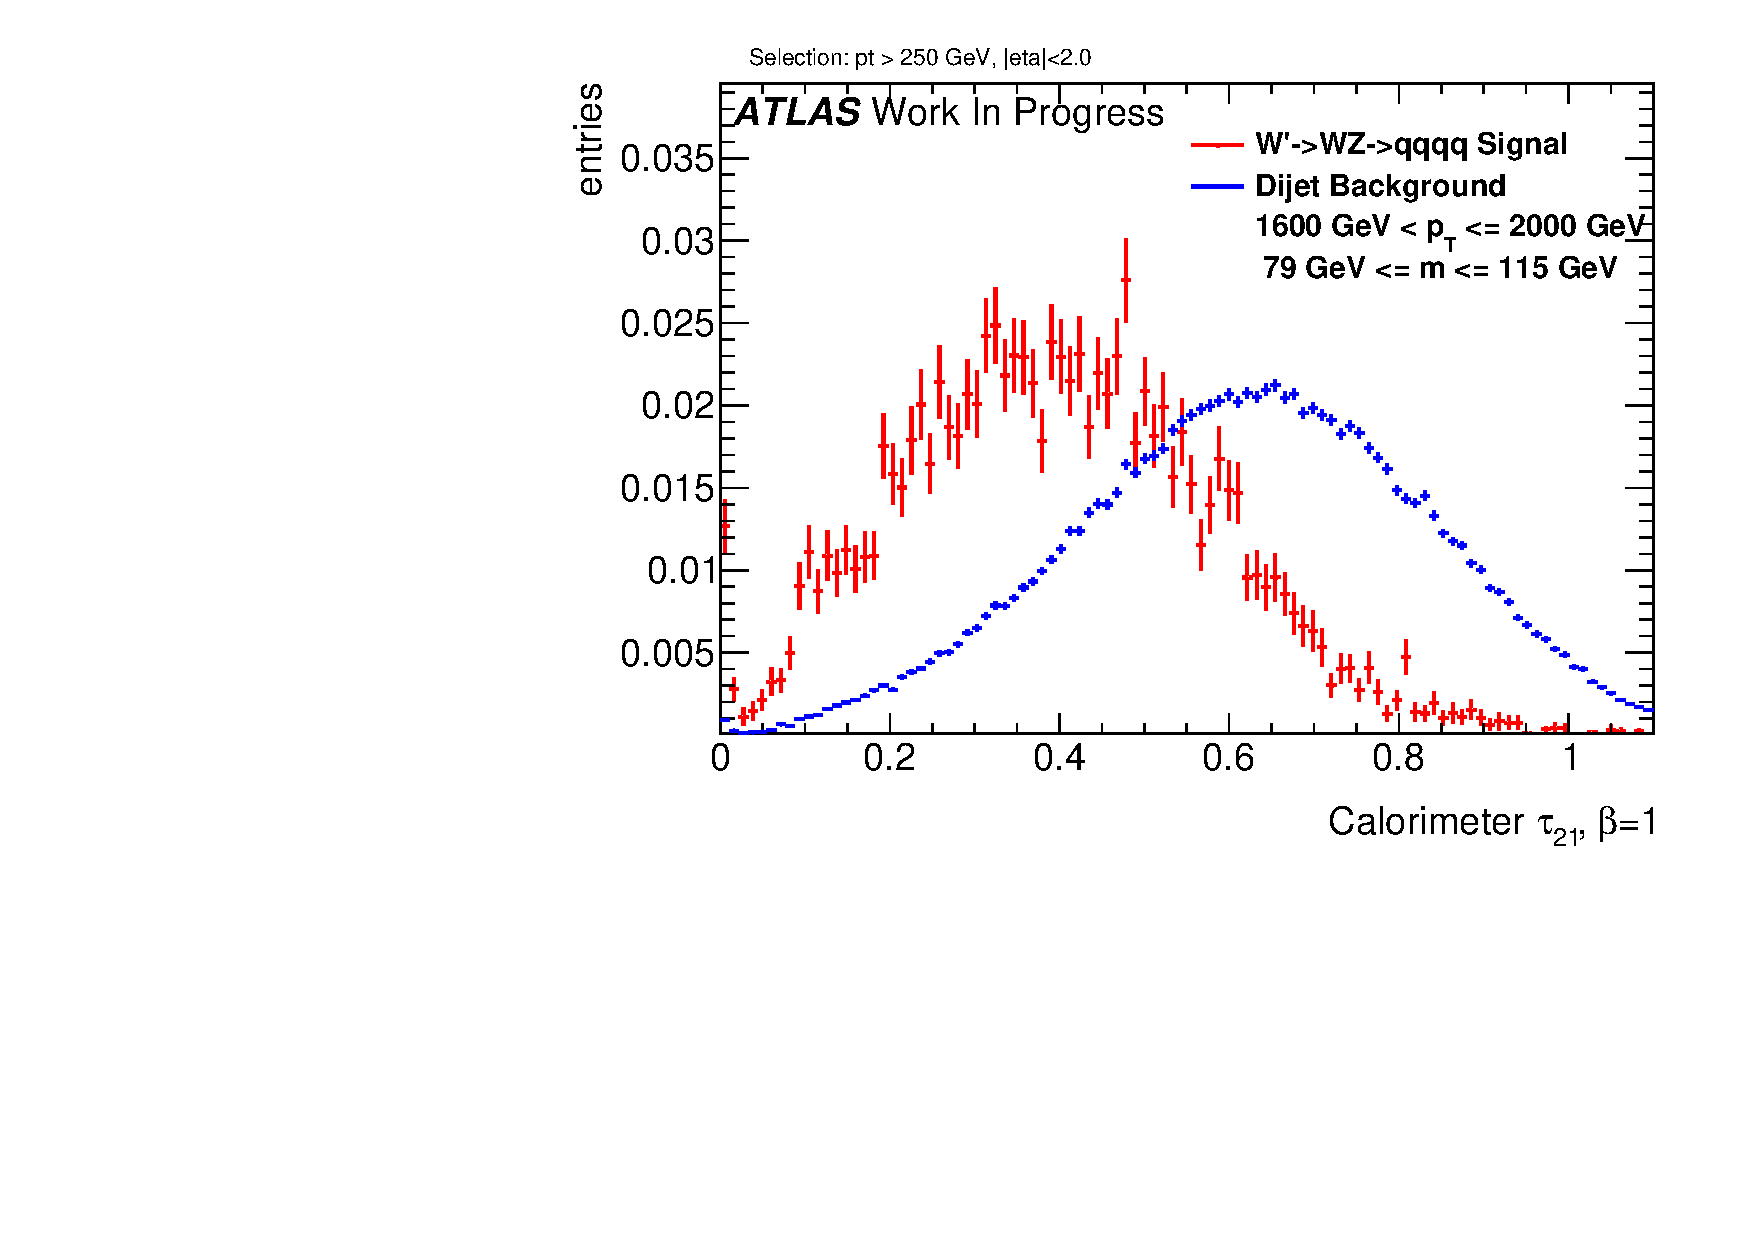
\includegraphics[width=0.3\textwidth]{sascha_input/plots/W/Beta1/h_recoJet_nSub21_bin5.pdf}
\bigskip
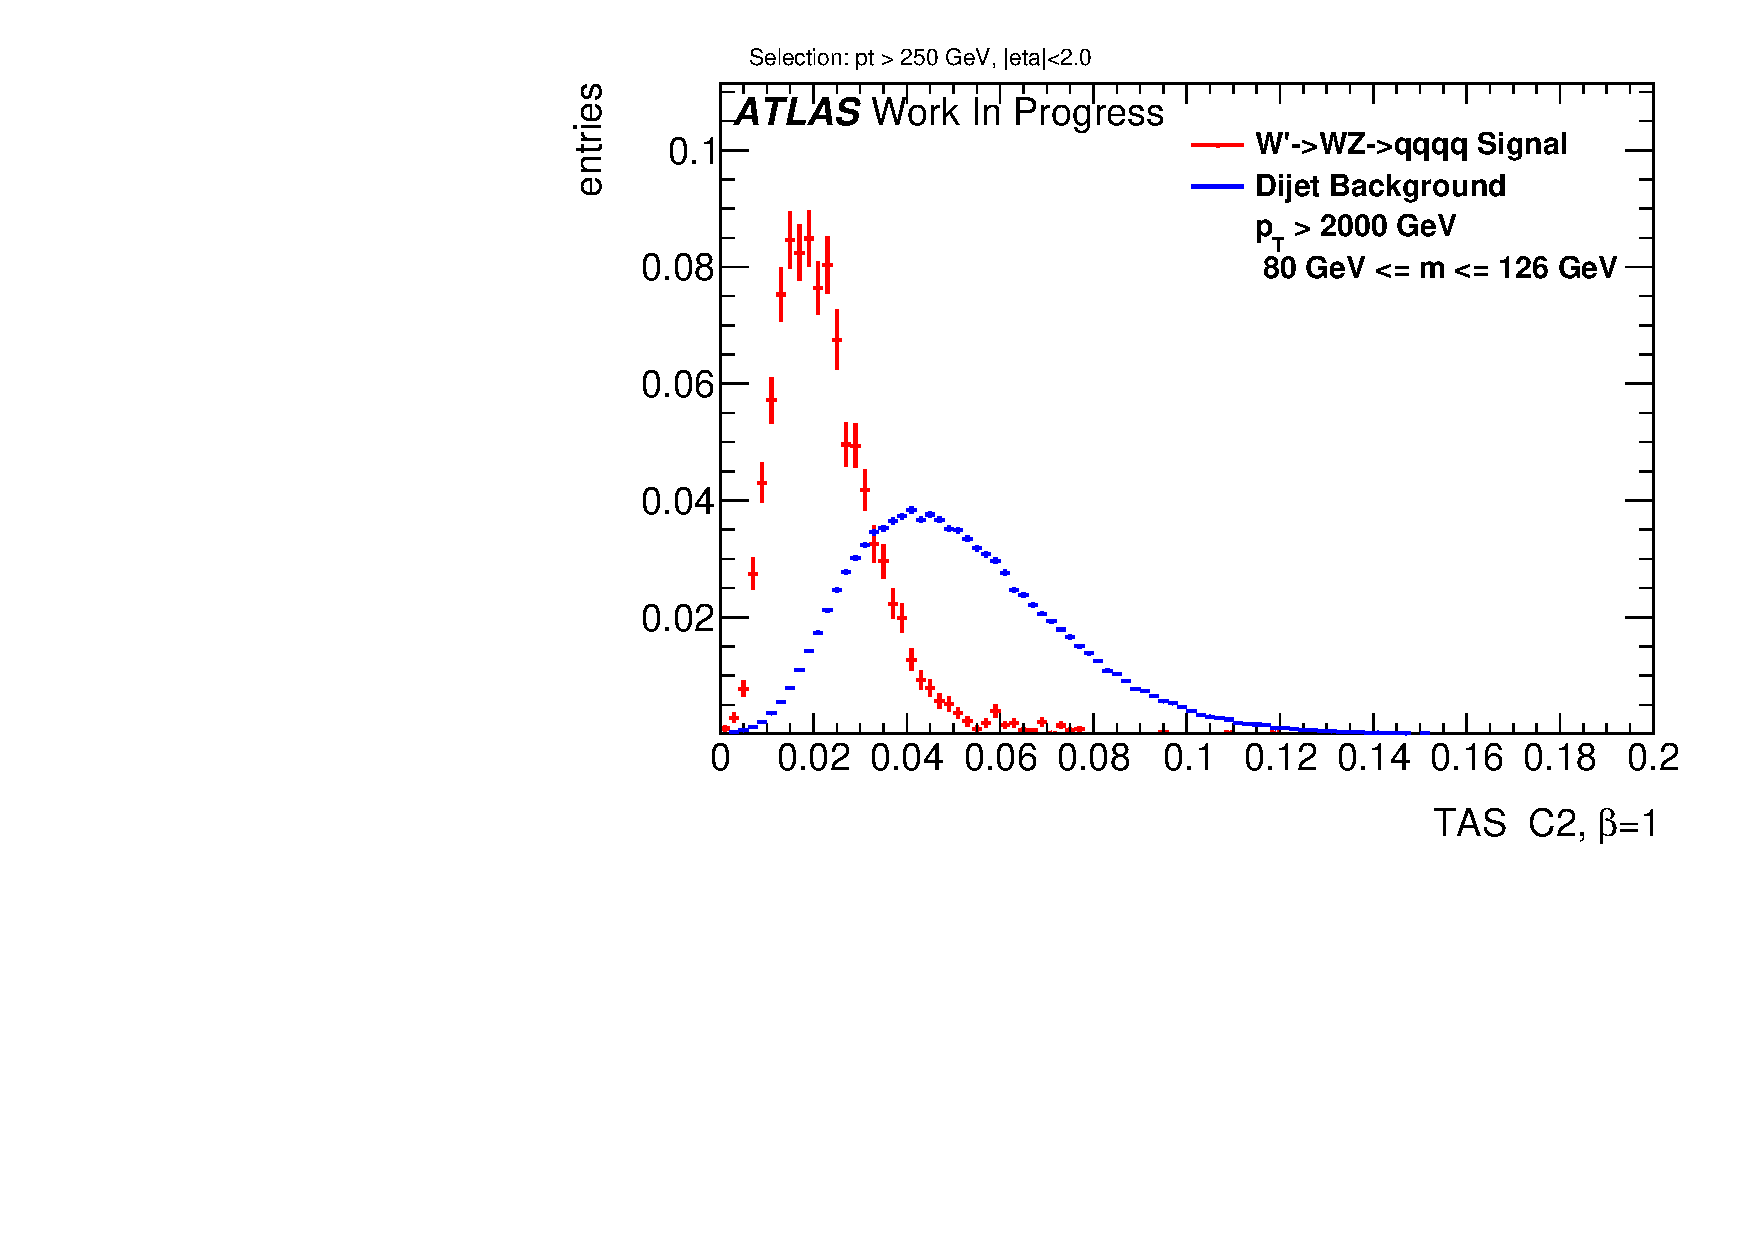
\includegraphics[width=0.3\textwidth]{sascha_input/plots/W/Beta1/h_assisted_tj_C2_bin6.pdf} \hspace{6mm}
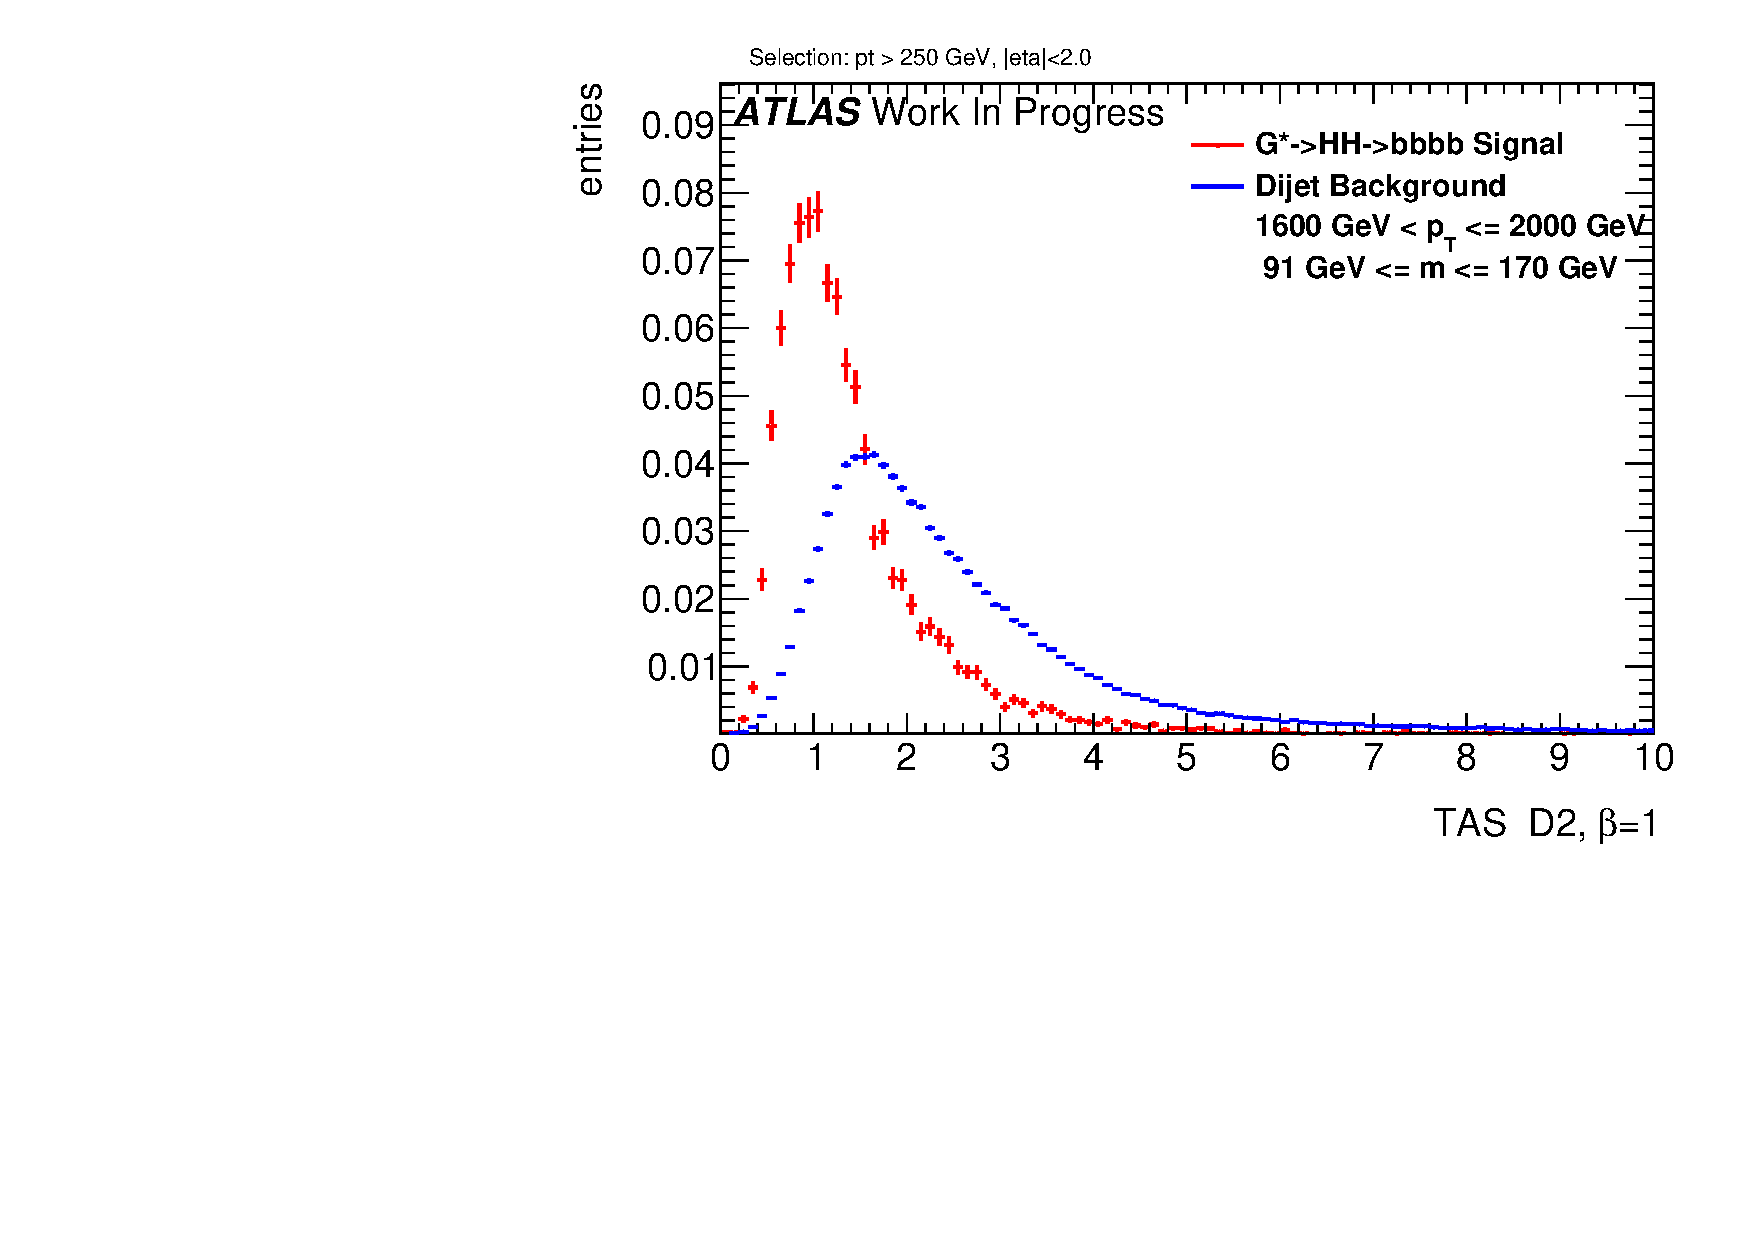
\includegraphics[width=0.3\textwidth]{sascha_input/plots/W/Beta1/h_assisted_tj_D2_bin5.pdf} \hspace{6mm}
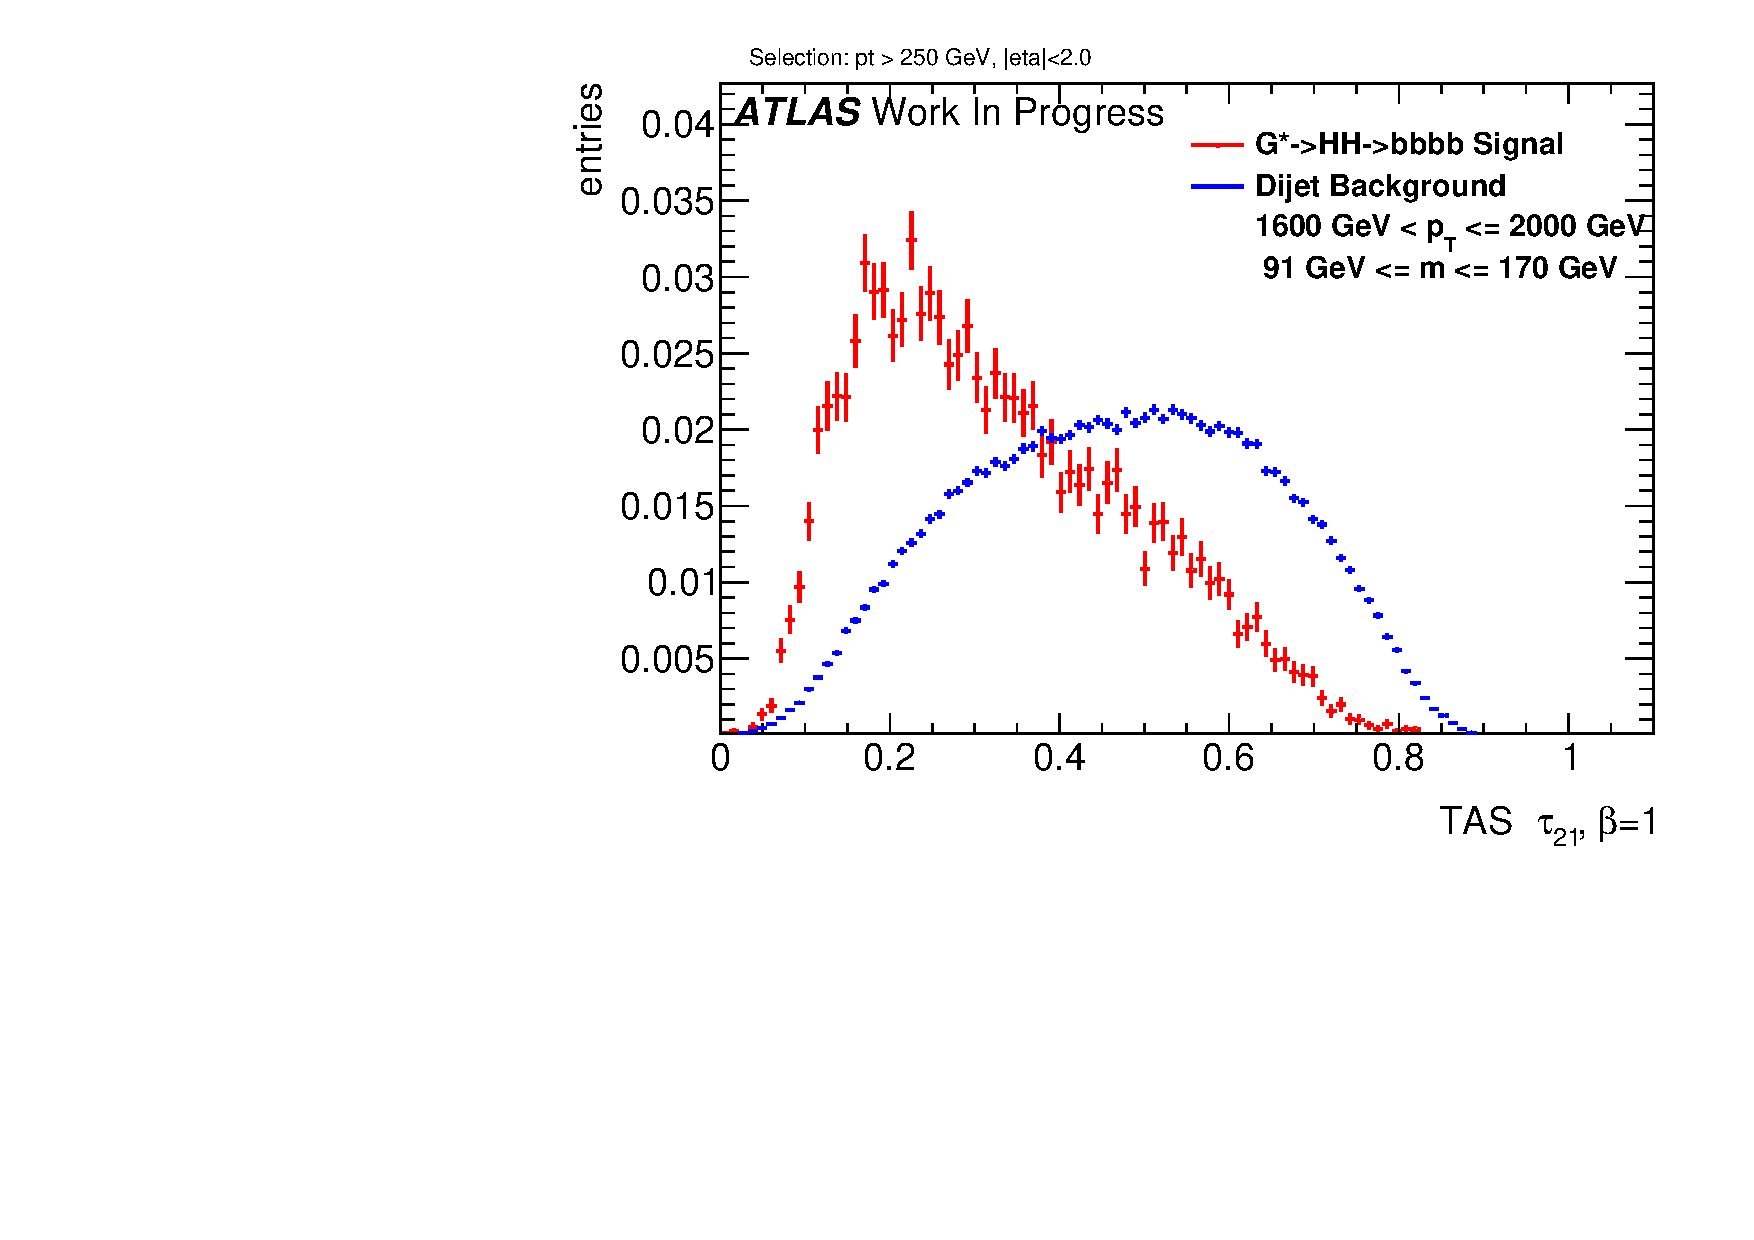
\includegraphics[width=0.3\textwidth]{sascha_input/plots/W/Beta1/h_assisted_tj_nSub21_bin5.pdf}
\caption{\footnotesize{$W$ boson signal and QCD background distributions for calorimeter (left) and TAS (right) at $\beta=1$  with C2 (top) for more than 2000 GeV and D2 (middle) and $\tau_{21}$ (bottom) for 1200-1600 GeV}}\label{fig:w_distribution_example}
\end{figure}

The ROCs in Figure \ref{fig:ROC_W_C2}, \ref{fig:ROC_W_D2} and \ref{fig:ROC_W_nSub21} show the actual achieved background rejection at different $p_T$ values. For lower $p_T$ values, TAS perform comparably to calorimeter clusters. Tracks without assisting achieve a considerably lower background rejection with D2 and $\tau_{21}$ for lower energies. Tracks and TAS perform equally well at high energies for D2 and $\tau_{21}$ and for C2 over the whole studied range. At higher boosts, the angular resolution of the tracks becomes more and more relevant as the separation between jet constituents shrinks. Consequently, tracks and TAS start to outperform calorimeter based variables and become increasingly effective with rising energy. 
\begin{figure}[htp]
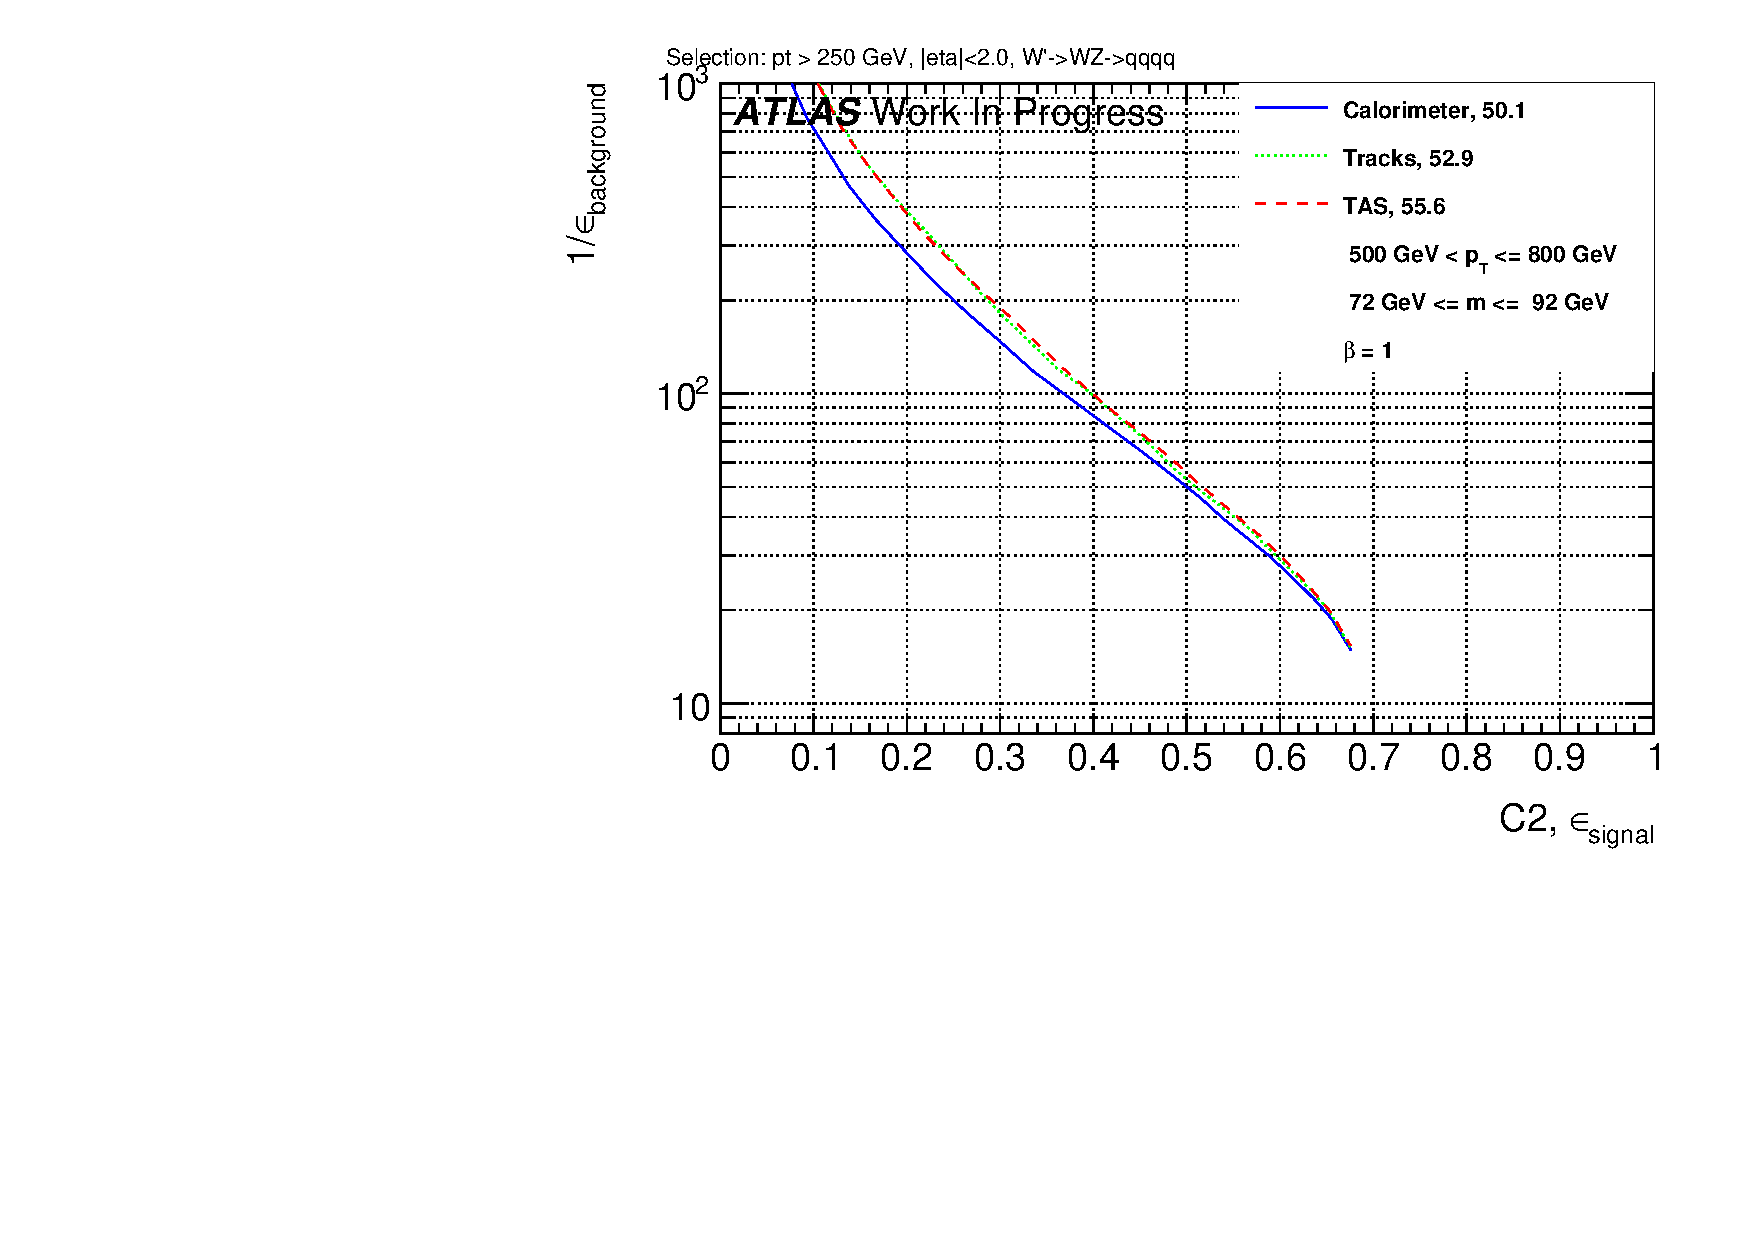
\includegraphics[width=0.5\textwidth]{sascha_input/plots/W/beta1/ROC_ALL_h_recoJet_C2_bin2.pdf} \hspace{1mm}
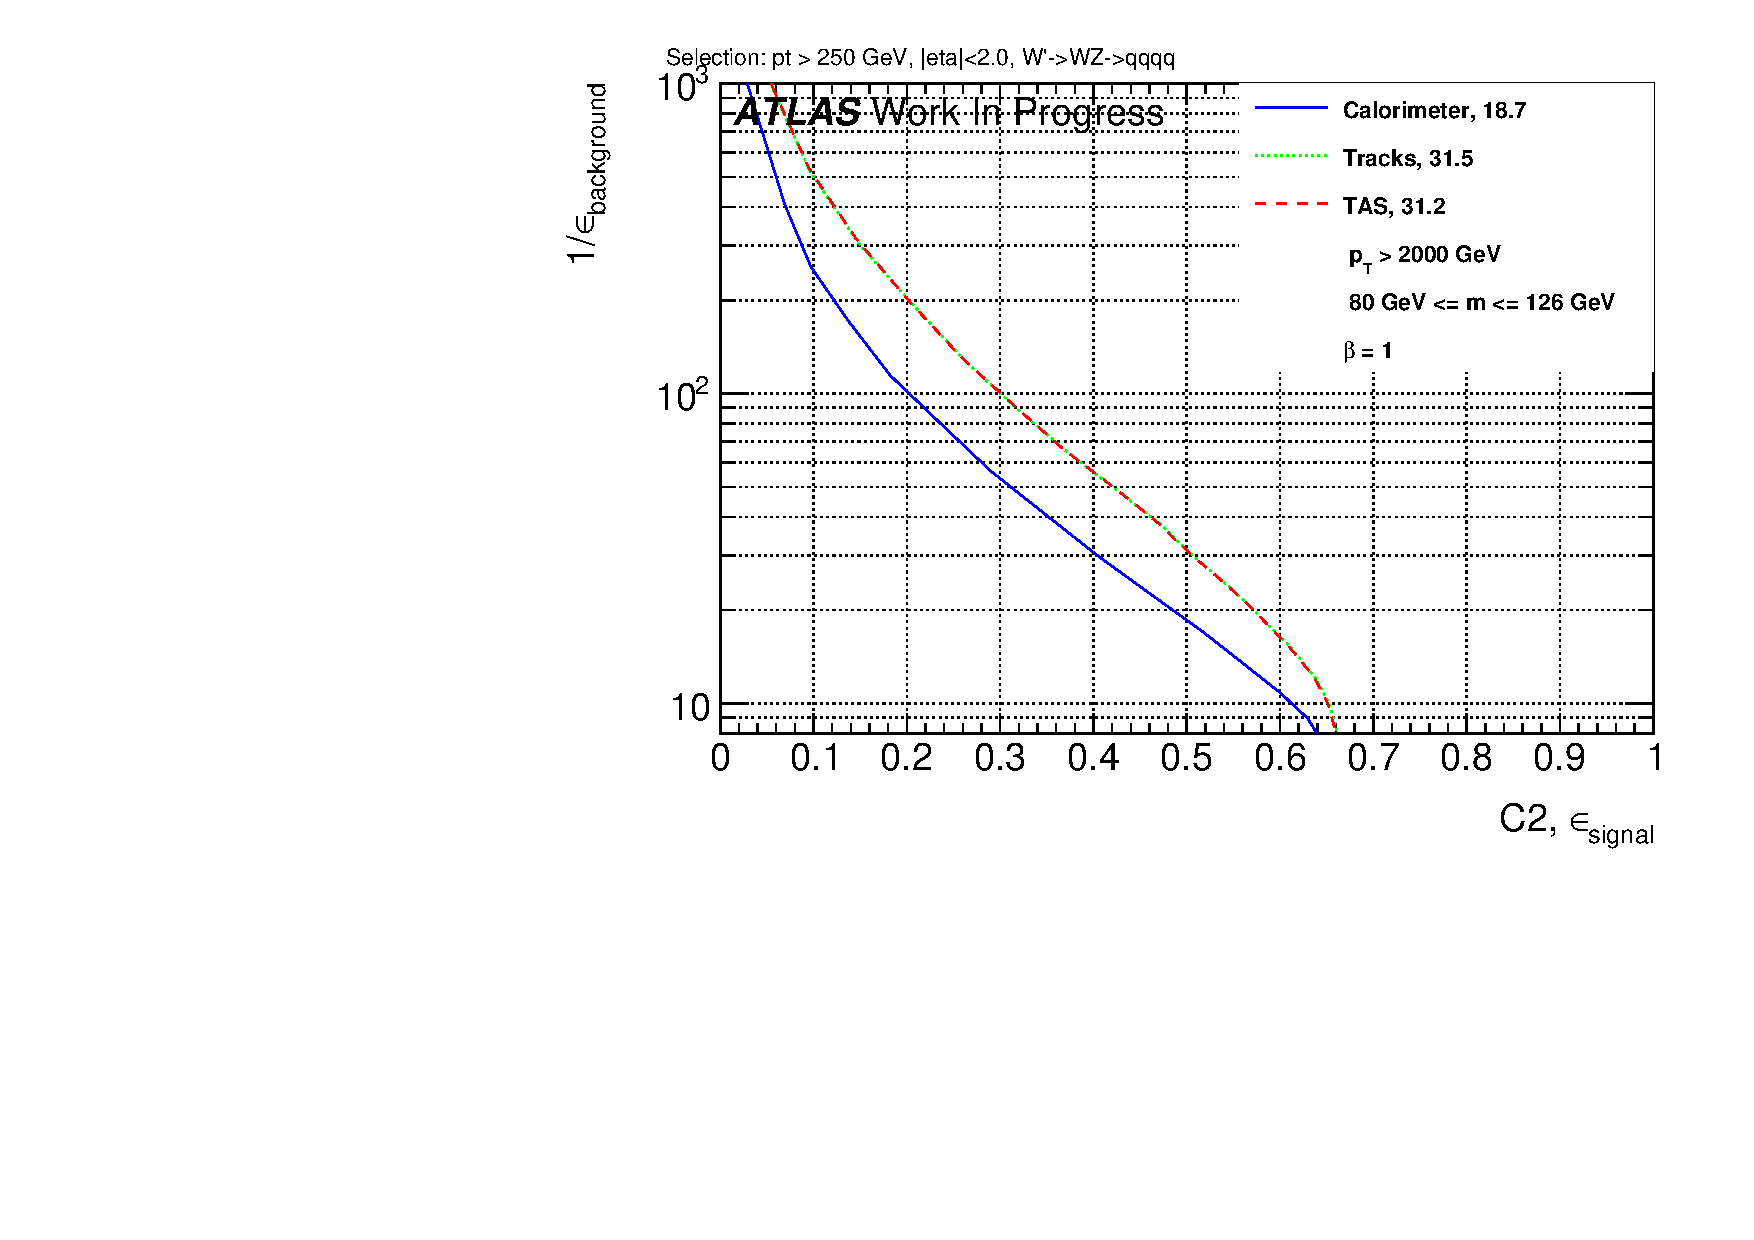
\includegraphics[width=0.5\textwidth]{sascha_input/plots/W/beta1/ROC_ALL_h_recoJet_C2_bin6.pdf}
\caption{\footnotesize{ROCs showing QCD rejection against $W$ boson efficiency for tracks, TAS and colorimeter C2 at $\beta=1$ for 500-800 GeV (left) and >2000 GeV (right). The numbers in the legend indicate the achieved background rejection at 50\% signal efficiency.}}\label{fig:ROC_W_C2}
\end{figure}

\begin{figure}[htp]
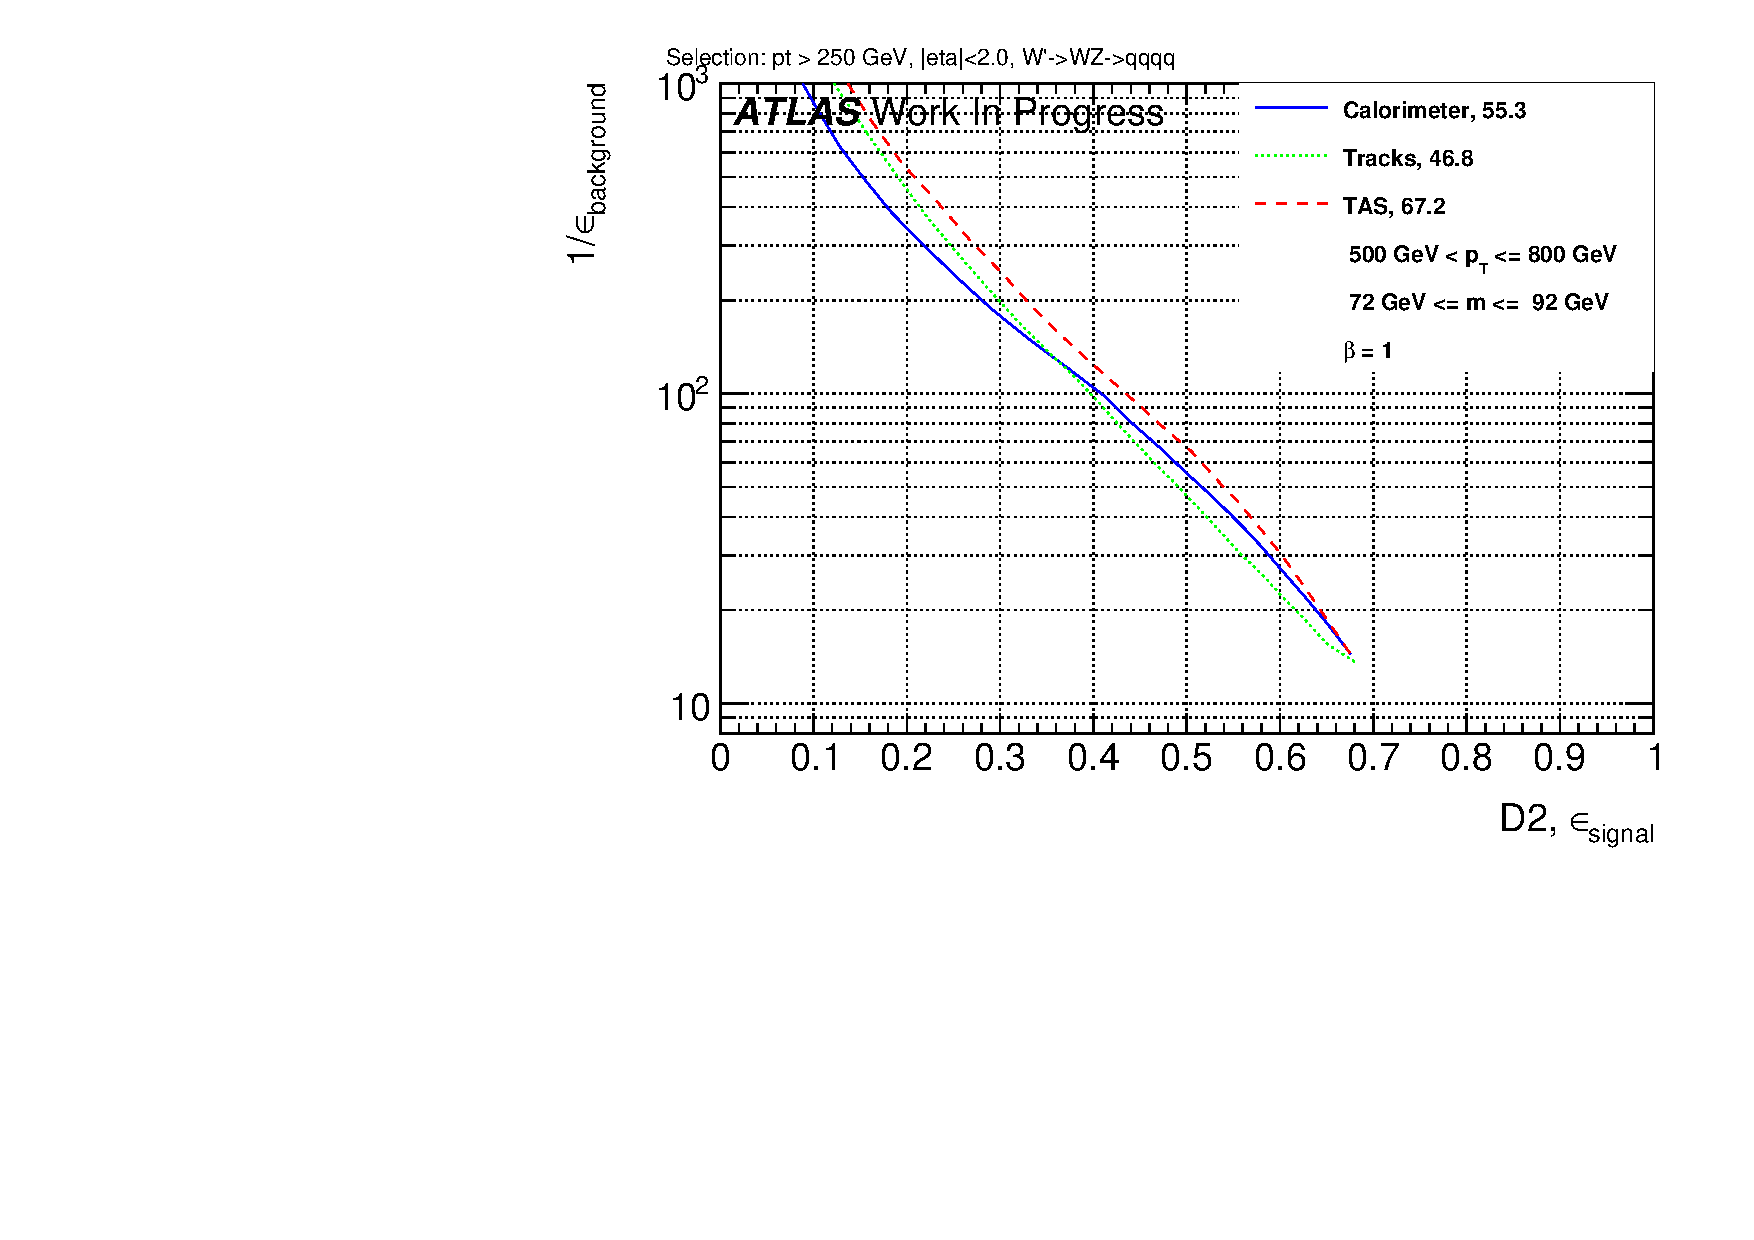
\includegraphics[width=0.5\textwidth]{sascha_input/plots/W/beta1/ROC_ALL_h_recoJet_D2_bin2.pdf}
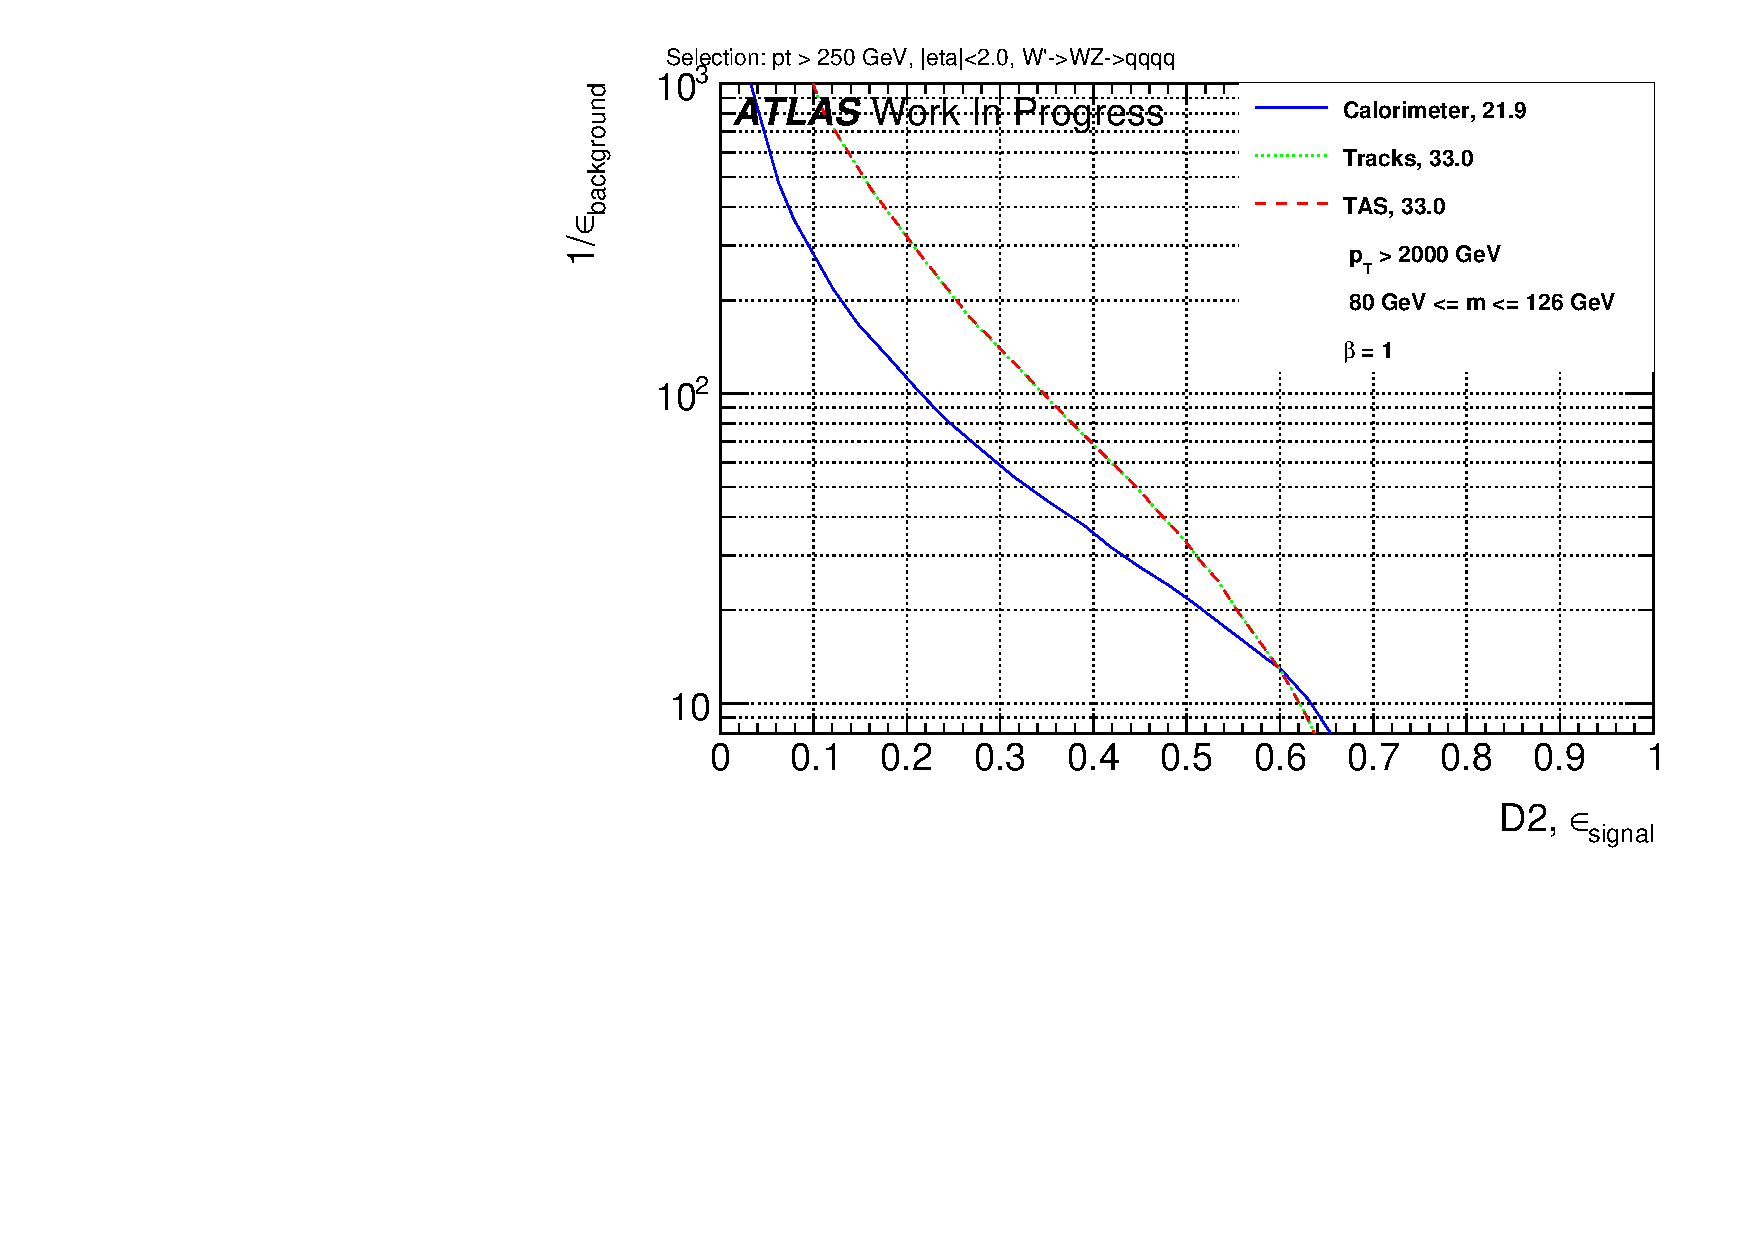
\includegraphics[width=0.5\textwidth]{sascha_input/plots/W/beta1/ROC_ALL_h_recoJet_D2_bin6.pdf}
\caption{\footnotesize{ROCs showing QCD rejection against $W$ boson efficiency for tracks, TAS and colorimeter D2 at $\beta=1$ for 500-800 GeV (left) and >2000 GeV (right). The numbers in the legend indicate the achieved background rejection at 50\% signal efficiency.}}\label{fig:ROC_W_D2}
\end{figure}

\begin{figure}[htp]
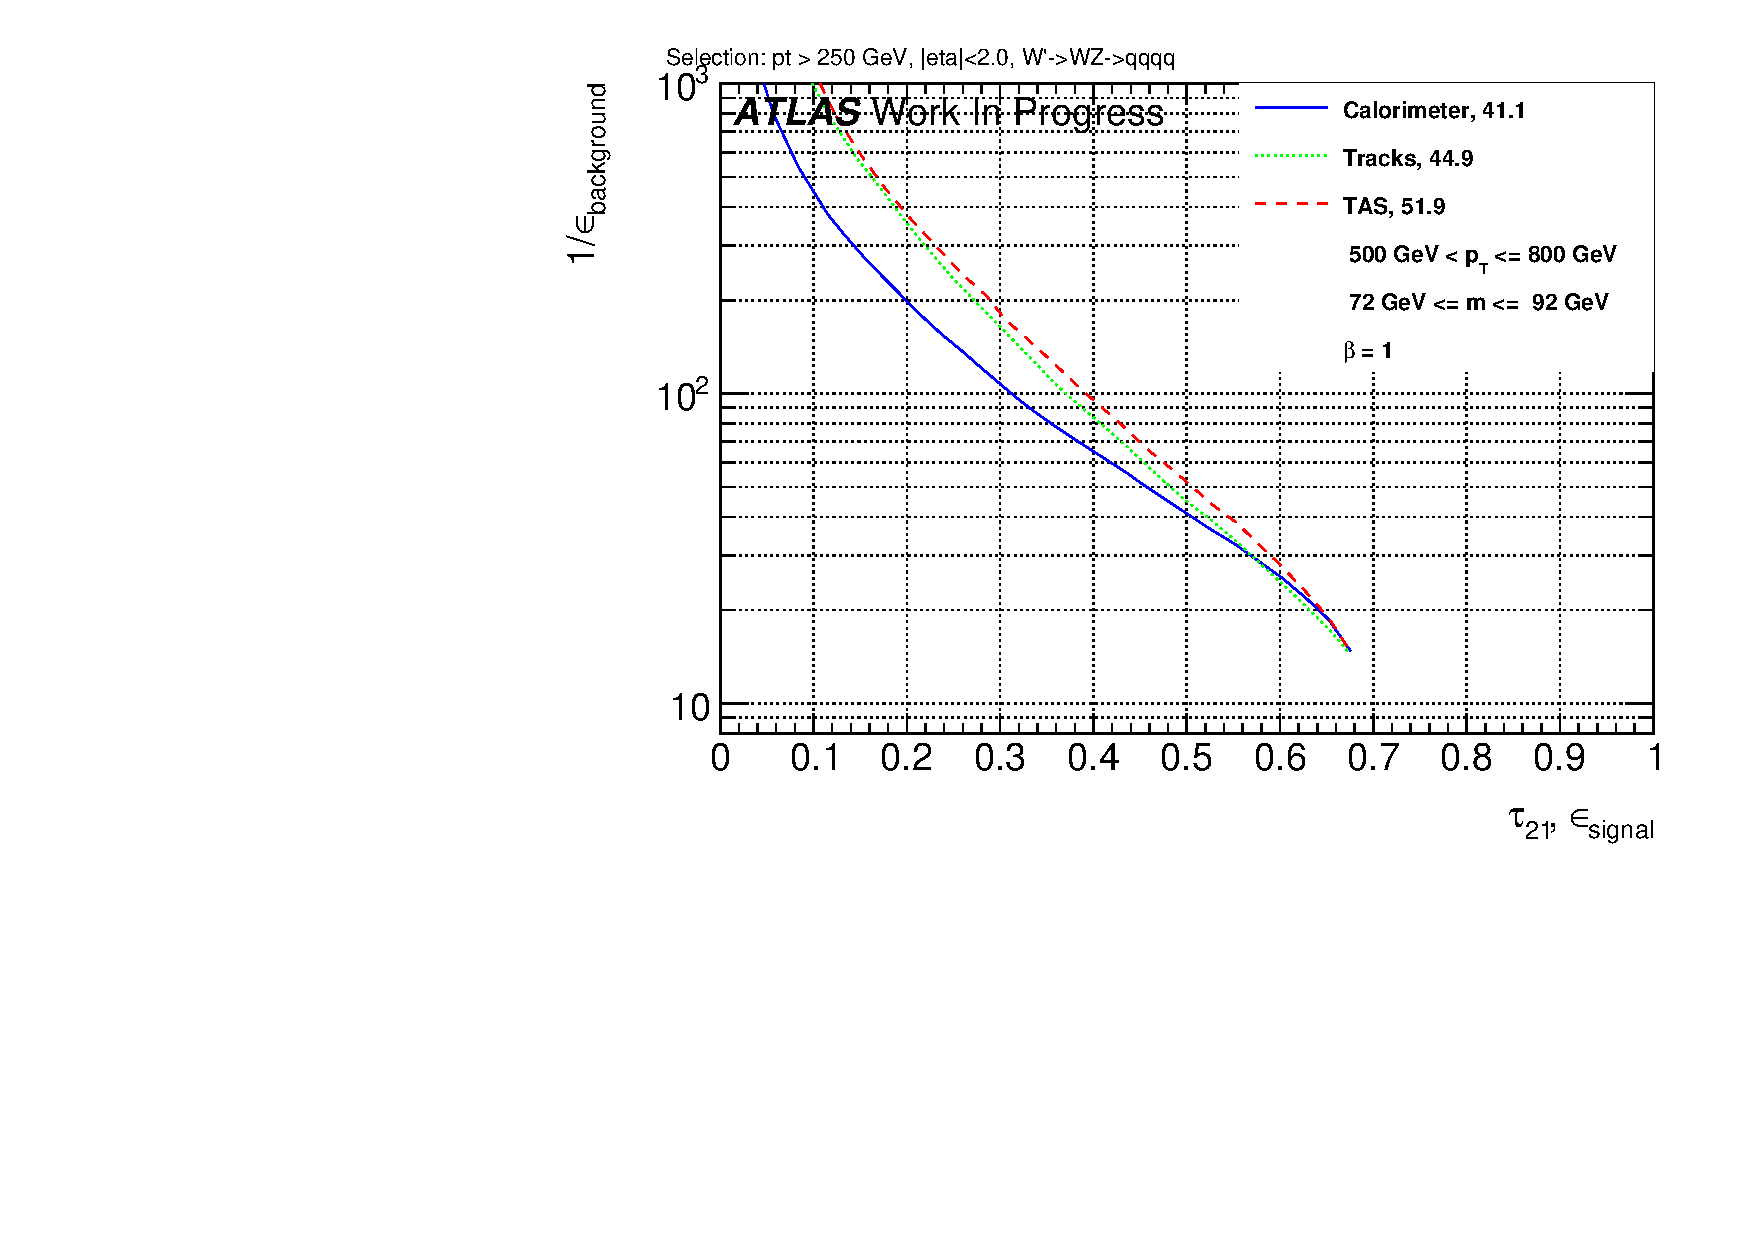
\includegraphics[width=0.5\textwidth]{sascha_input/plots/W/beta1/ROC_ALL_h_recoJet_nSub21_bin2.pdf}
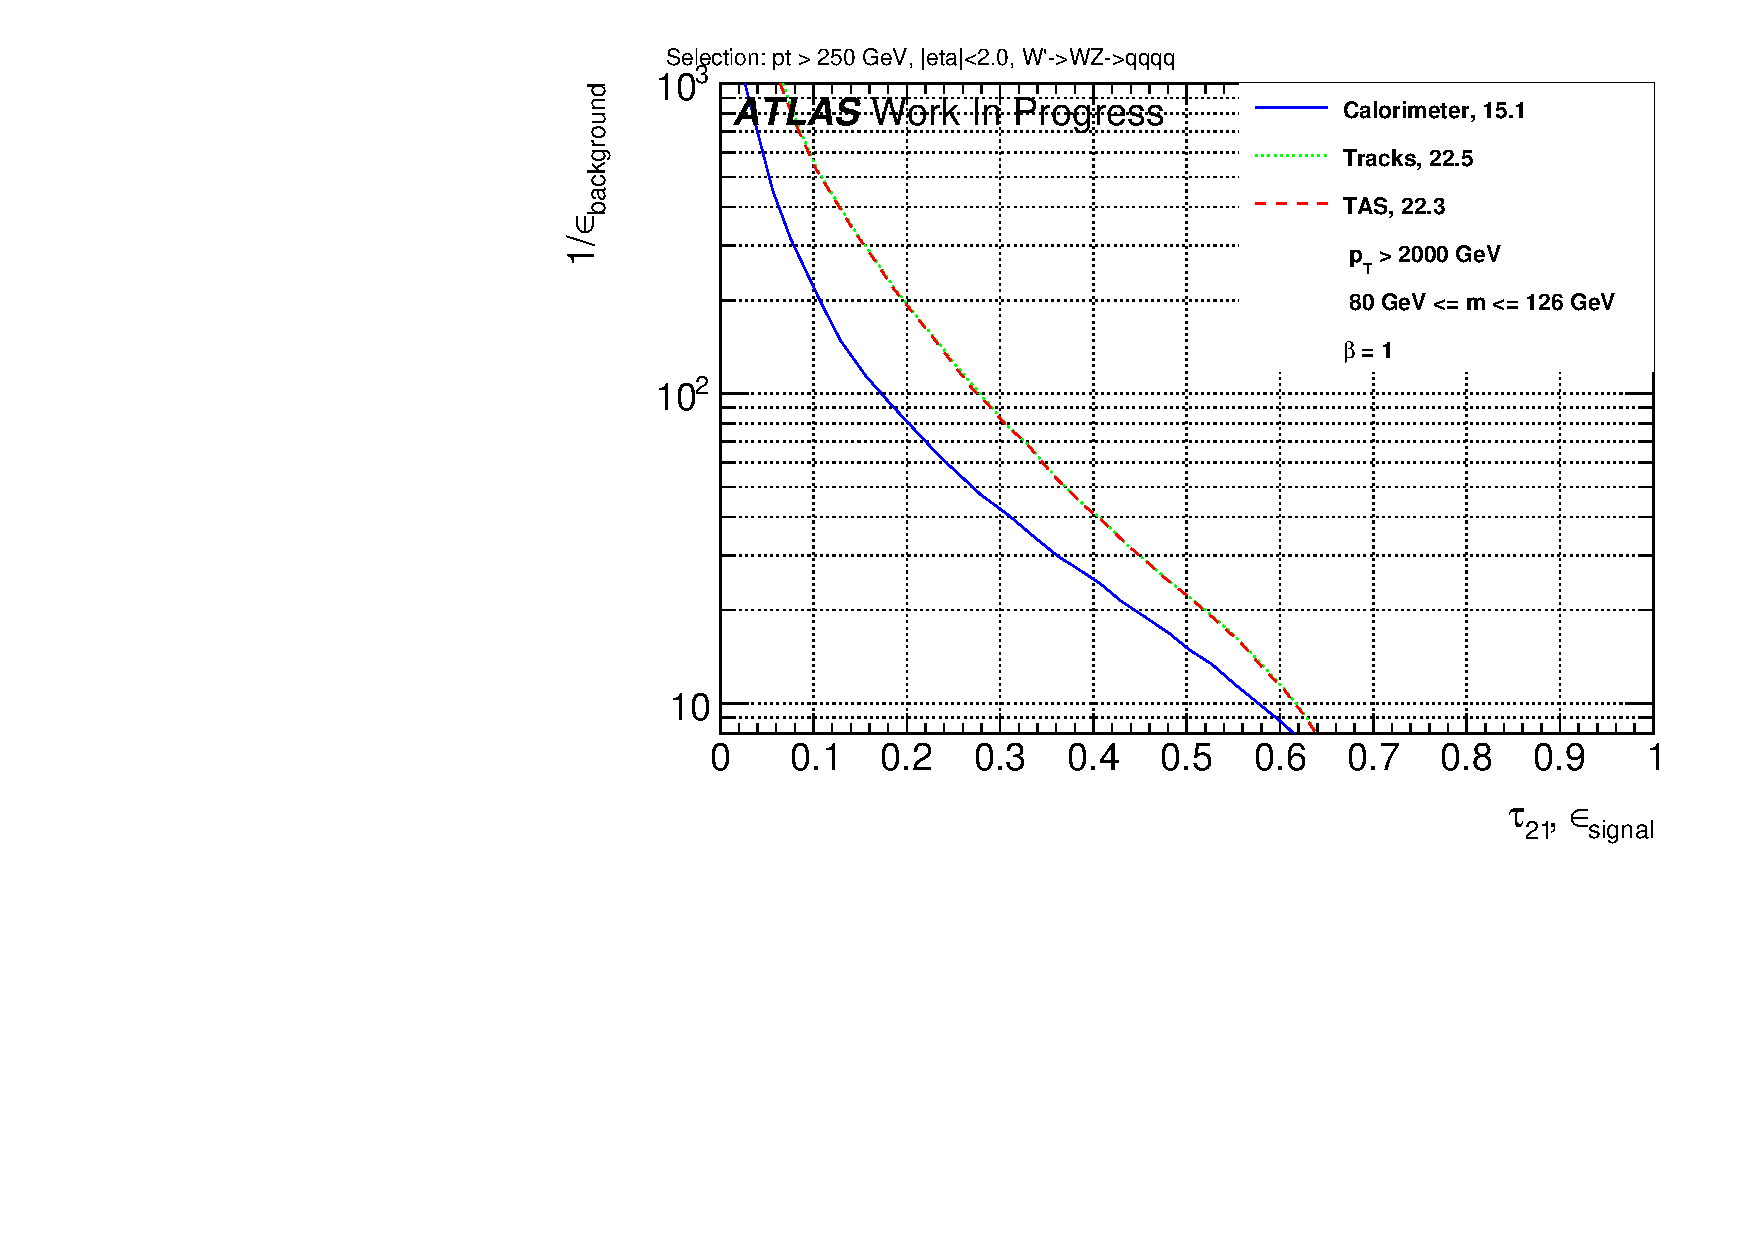
\includegraphics[width=0.5\textwidth]{sascha_input/plots/W/beta1/ROC_ALL_h_recoJet_nSub21_bin6.pdf}
\caption{\footnotesize{ROCs showing QCD rejection against $W$ boson efficiency for tracks, TAS and colorimeter $\tau_{21}$ at $\beta=1$ for 500-800 GeV (left) and >2000 GeV (right). The numbers in the legend indicate the achieved background rejection at 50\% signal efficiency.}}\label{fig:ROC_W_nSub21}
\end{figure}

\subsubsection{Un-assisted tracks and TAS at very high $p_{\mathrm{T}}$}
The C2 variable was found to perform equally well with tracks and TAS as input. This variable seems to be relative insensitive to the track assisting and tracks alone already perform well. D2 and $\tau_{21}$ in contrast, feature a visibly worse separation with tracks than with assisted tracks. In these cases, the scale difference due to the missing neutral fraction seems to have a greater influence.

For very high $p_{\mathrm{T}}$ values however, it is often the case that the large-R calorimeter jet features only one $R = 0.2$ sub-jet after trimming due to the now small separation of constituents. A single sub-jet results in the TAS procedure to fall back to TA. As stated in Section \ref{subsec:ta_adapt}, TA has no impact on the ratios. Therefore, C2/D2 and $\tau_{21}$ perform equally well when calculated with tracks or TAS for events with only one sub-jet and thereby the difference between both decreases for very high energies. 


\subsubsection{Correlation with $p_{\mathrm{T}}$}
Due to the rapidly falling $p_{\mathrm{T}}$ spectrum and hence low weights for high $p_{\mathrm{T}}$ are the correlation plots divided into the six different $p_{\mathrm{T}}$ regions.
For C2, see Figure \ref{fig:correlation_C2}, one can observe a strong trend to lower values for signal and background with calorimeter clusters as well as TAS. Furthermore, it is possible to observe that the TAS distributions concentrate at lower values compared to calorimeter counterparts.

In the cases of D2, Figure \ref{fig:correlation_D2}, and $\tau_{21}$, Figure \ref{fig:correlation_tau21}, there is a small upward trend of the calorimeter variables visible in the lower $p_{\mathrm{T}}$ regions which, with rising boost, slows down for D2 and $\tau_{21}$ and ends for $\tau_{21}$ in a broader distribution. This verifies the higher $p_{\mathrm{T}}$ dependence of the C2 variable in comparison to D2 and $\tau_{21}$. The TAS counterparts feature an even more robust signal with the background moving to higher values, hence improving separation. The $p_{\mathrm{T}}$ dependence of variables calculated with tracks is very similar to the ones with TAS, therefore they are omitted.

\begin{figure}[htp]
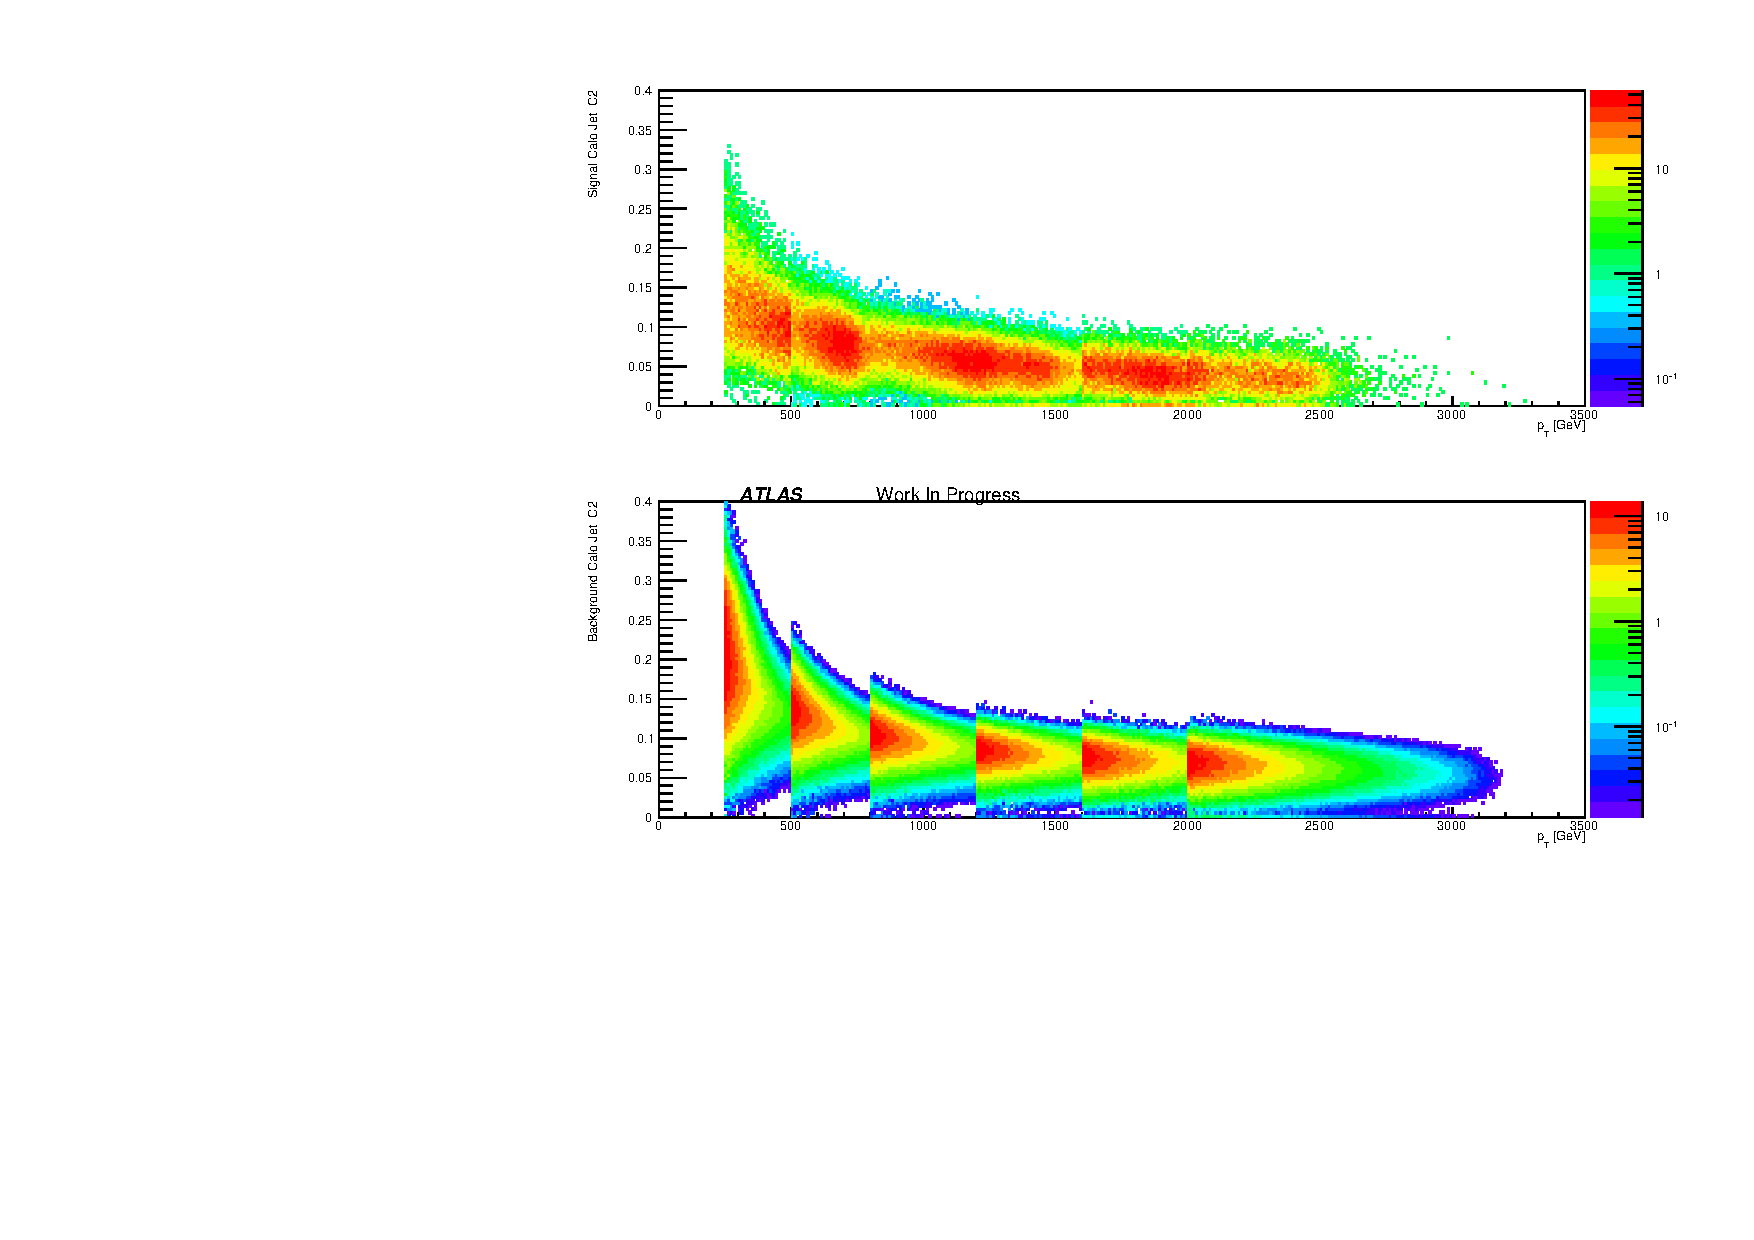
\includegraphics[width=0.5\textwidth]{sascha_input/plots/W/beta1/scatter_plots/scatter_h_scatter_reco_C2.pdf}
\bigskip
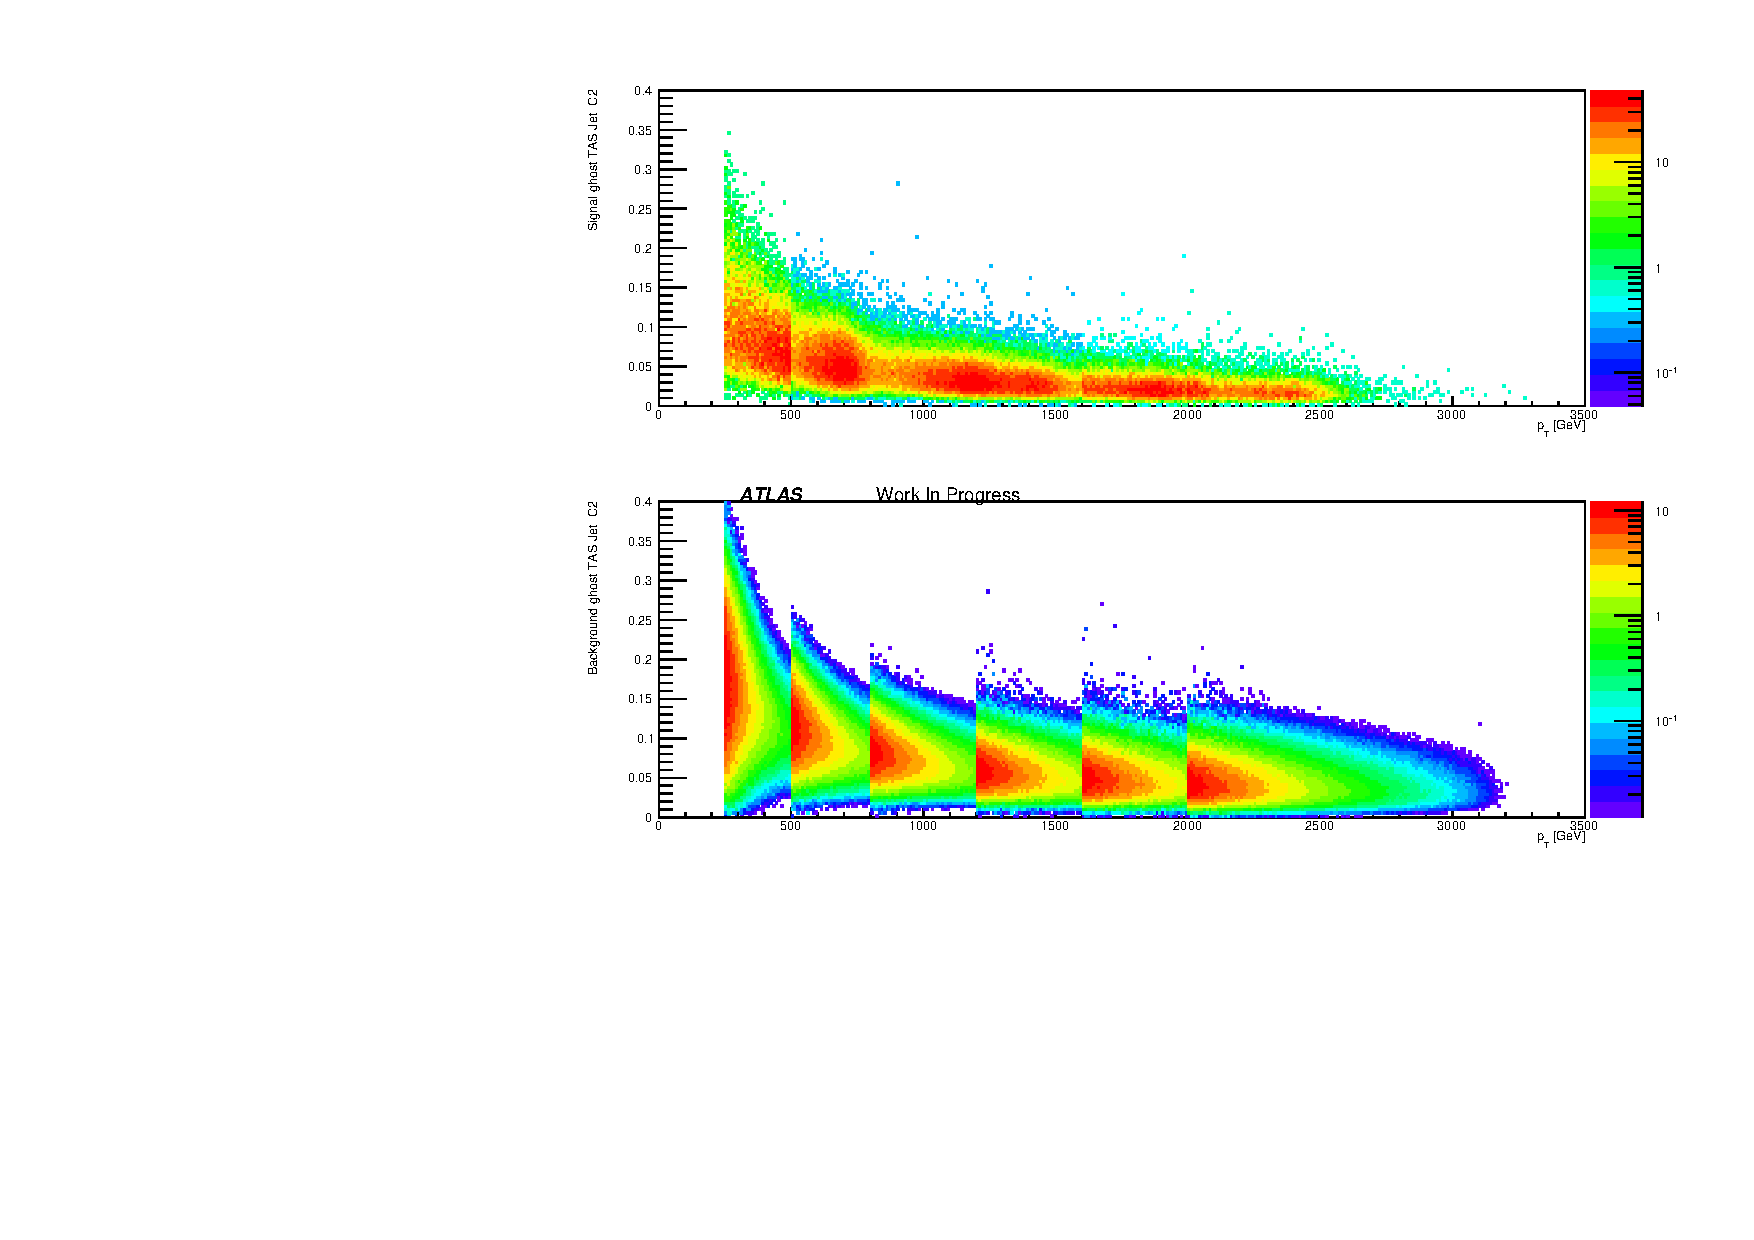
\includegraphics[width=0.5\textwidth]{sascha_input/plots/W/beta1/scatter_plots/scatter_h_scatter_assisted_tj_C2.pdf} 
\caption{\footnotesize{Correlation between C2 at $\beta=1$ and $p_{\mathrm{T}}$ applied on $W$ boson signal (above) and QCD background (below) for calorimeter (left) and TAS (right).}}\label{fig:correlation_C2}
\end{figure}

\begin{figure}[htp]
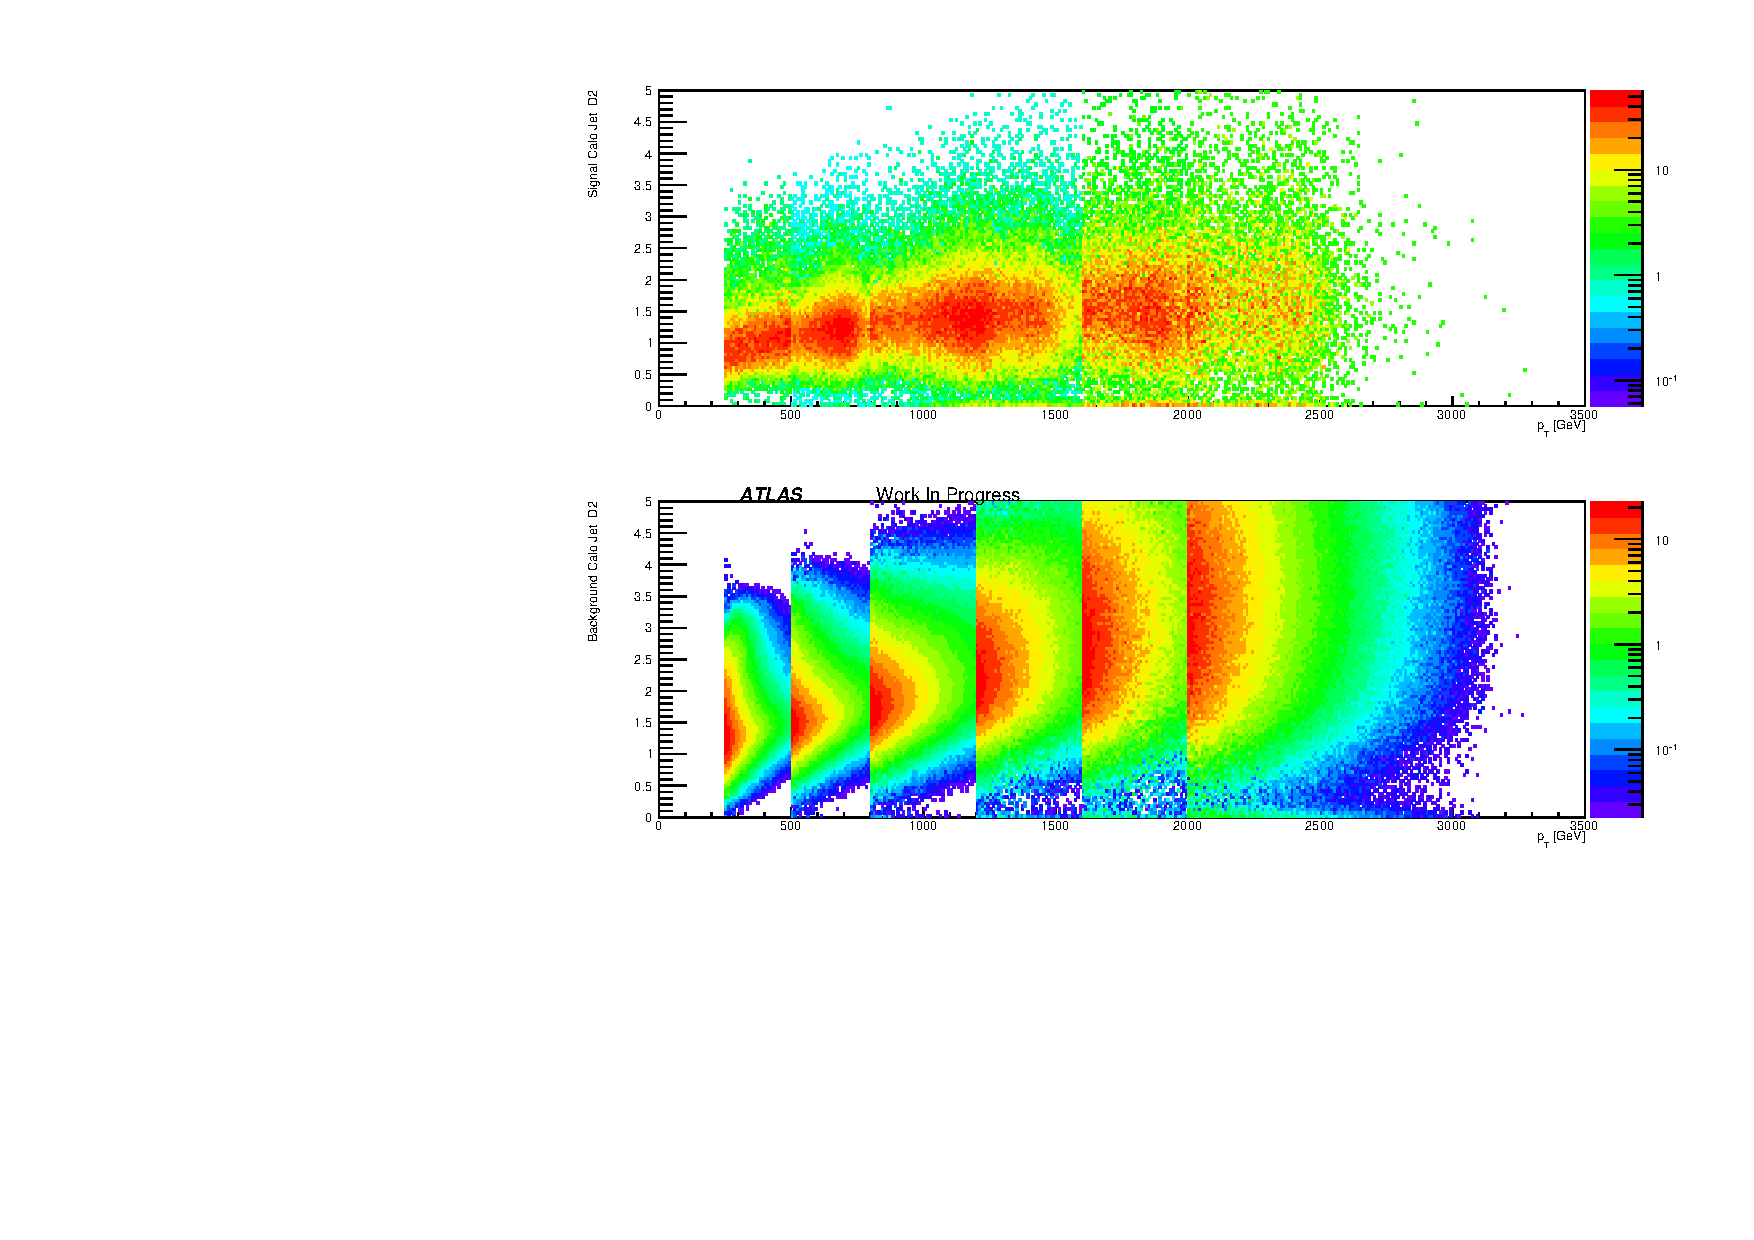
\includegraphics[width=0.5\textwidth]{sascha_input/plots/W/beta1/scatter_plots/scatter_h_scatter_reco_D2.pdf}
\bigskip
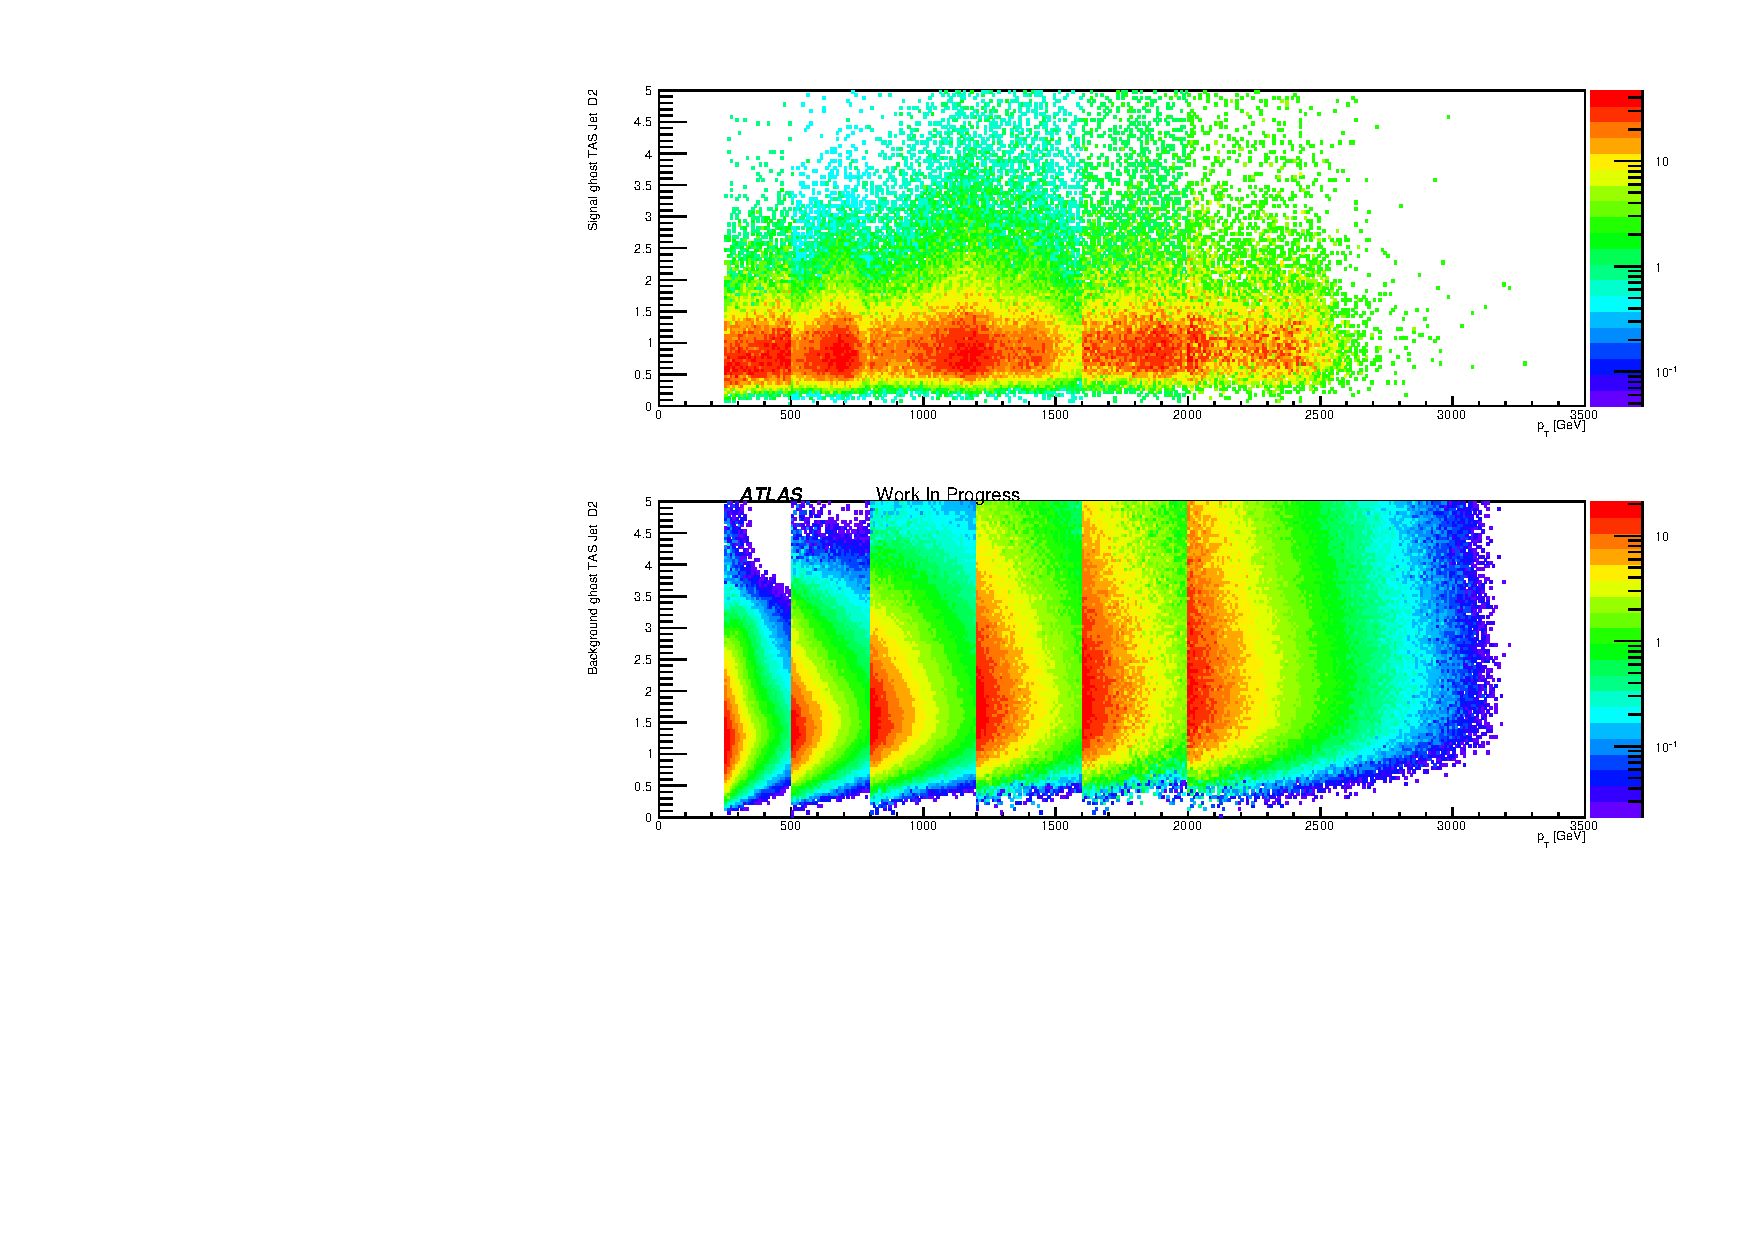
\includegraphics[width=0.5\textwidth]{sascha_input/plots/W/beta1/scatter_plots/scatter_h_scatter_assisted_tj_D2.pdf} 
\caption{\footnotesize{Correlation between D2 at $\beta=1$ and $p_{\mathrm{T}}$ applied on $W$ boson signal (above) and QCD background (below) for calorimeter (left) and TAS (right).}}\label{fig:correlation_D2}
\end{figure}

\begin{figure}[htp]
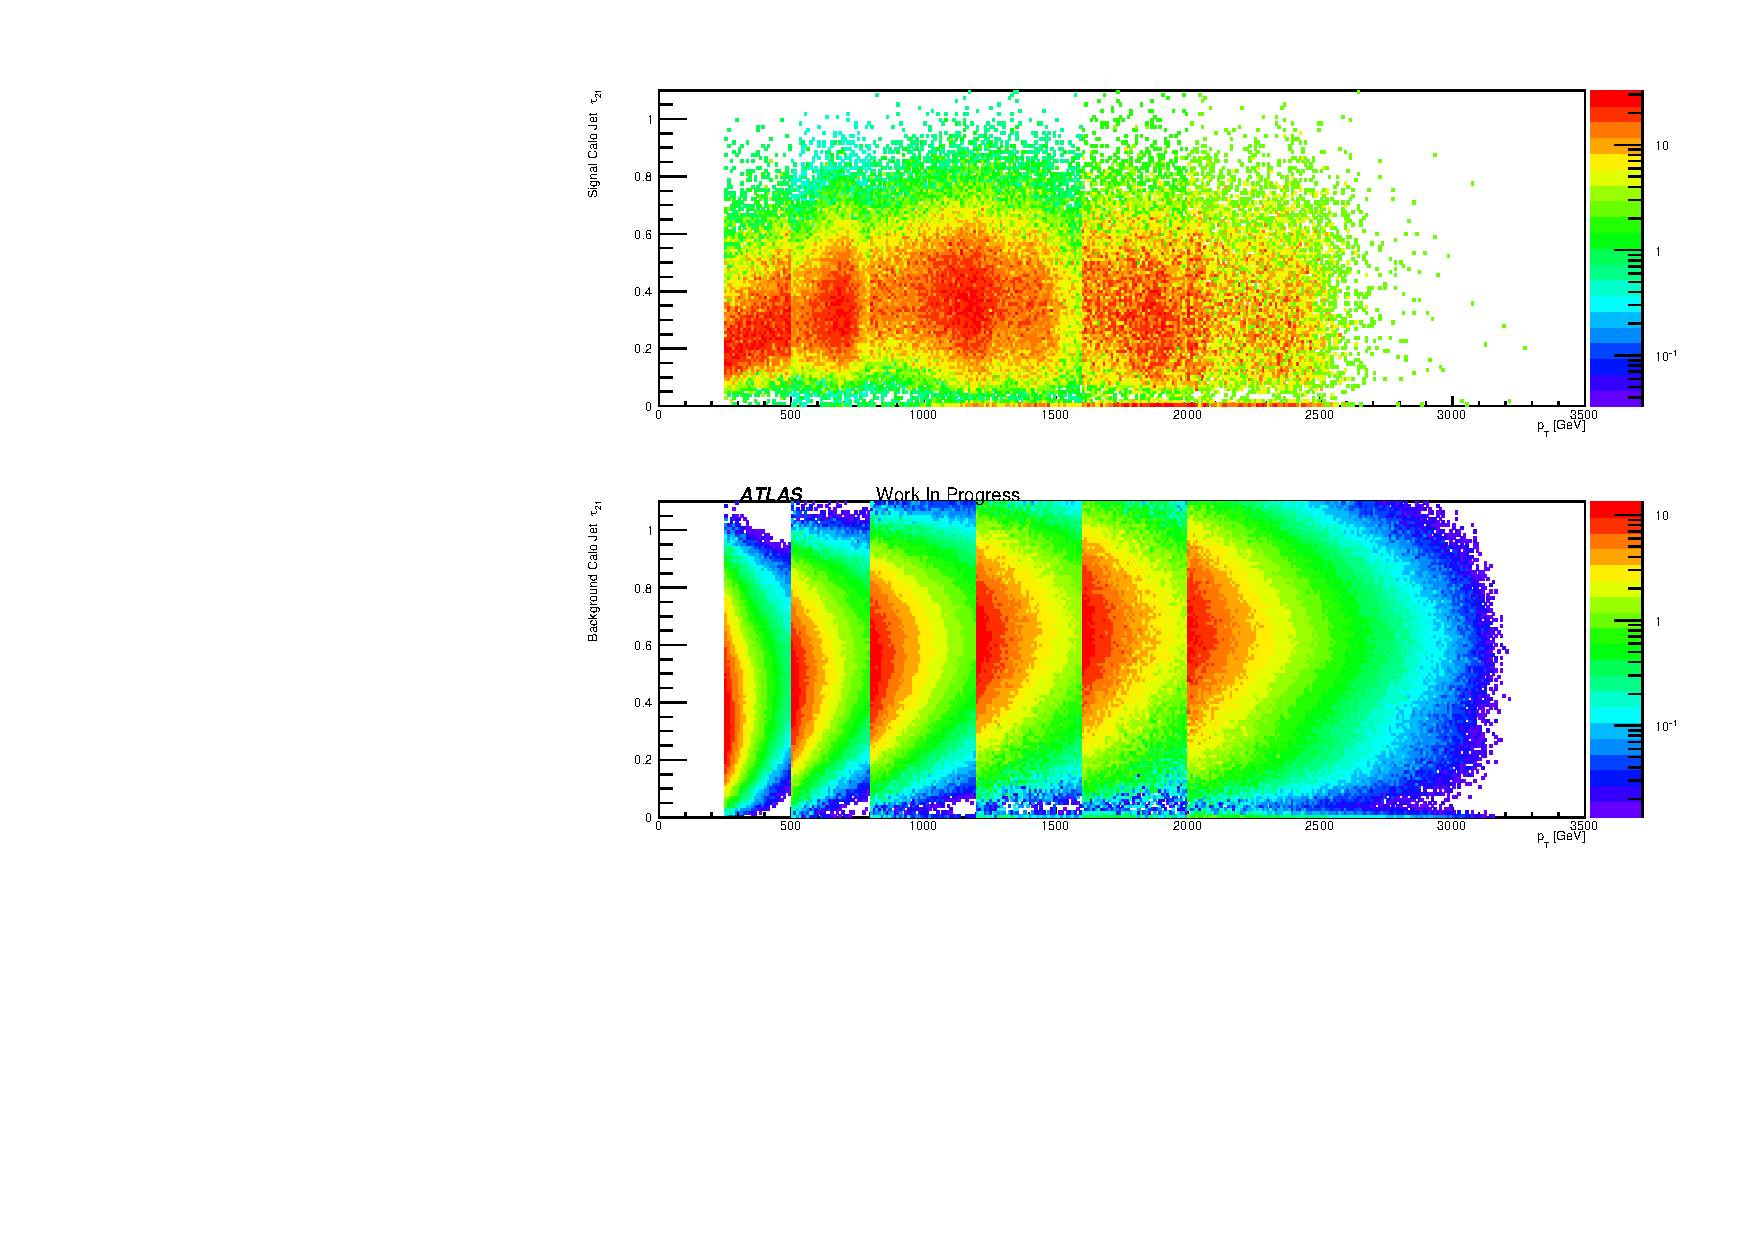
\includegraphics[width=0.5\textwidth]{sascha_input/plots/W/beta1/scatter_plots/scatter_h_scatter_reco_nSub21.pdf}
\bigskip
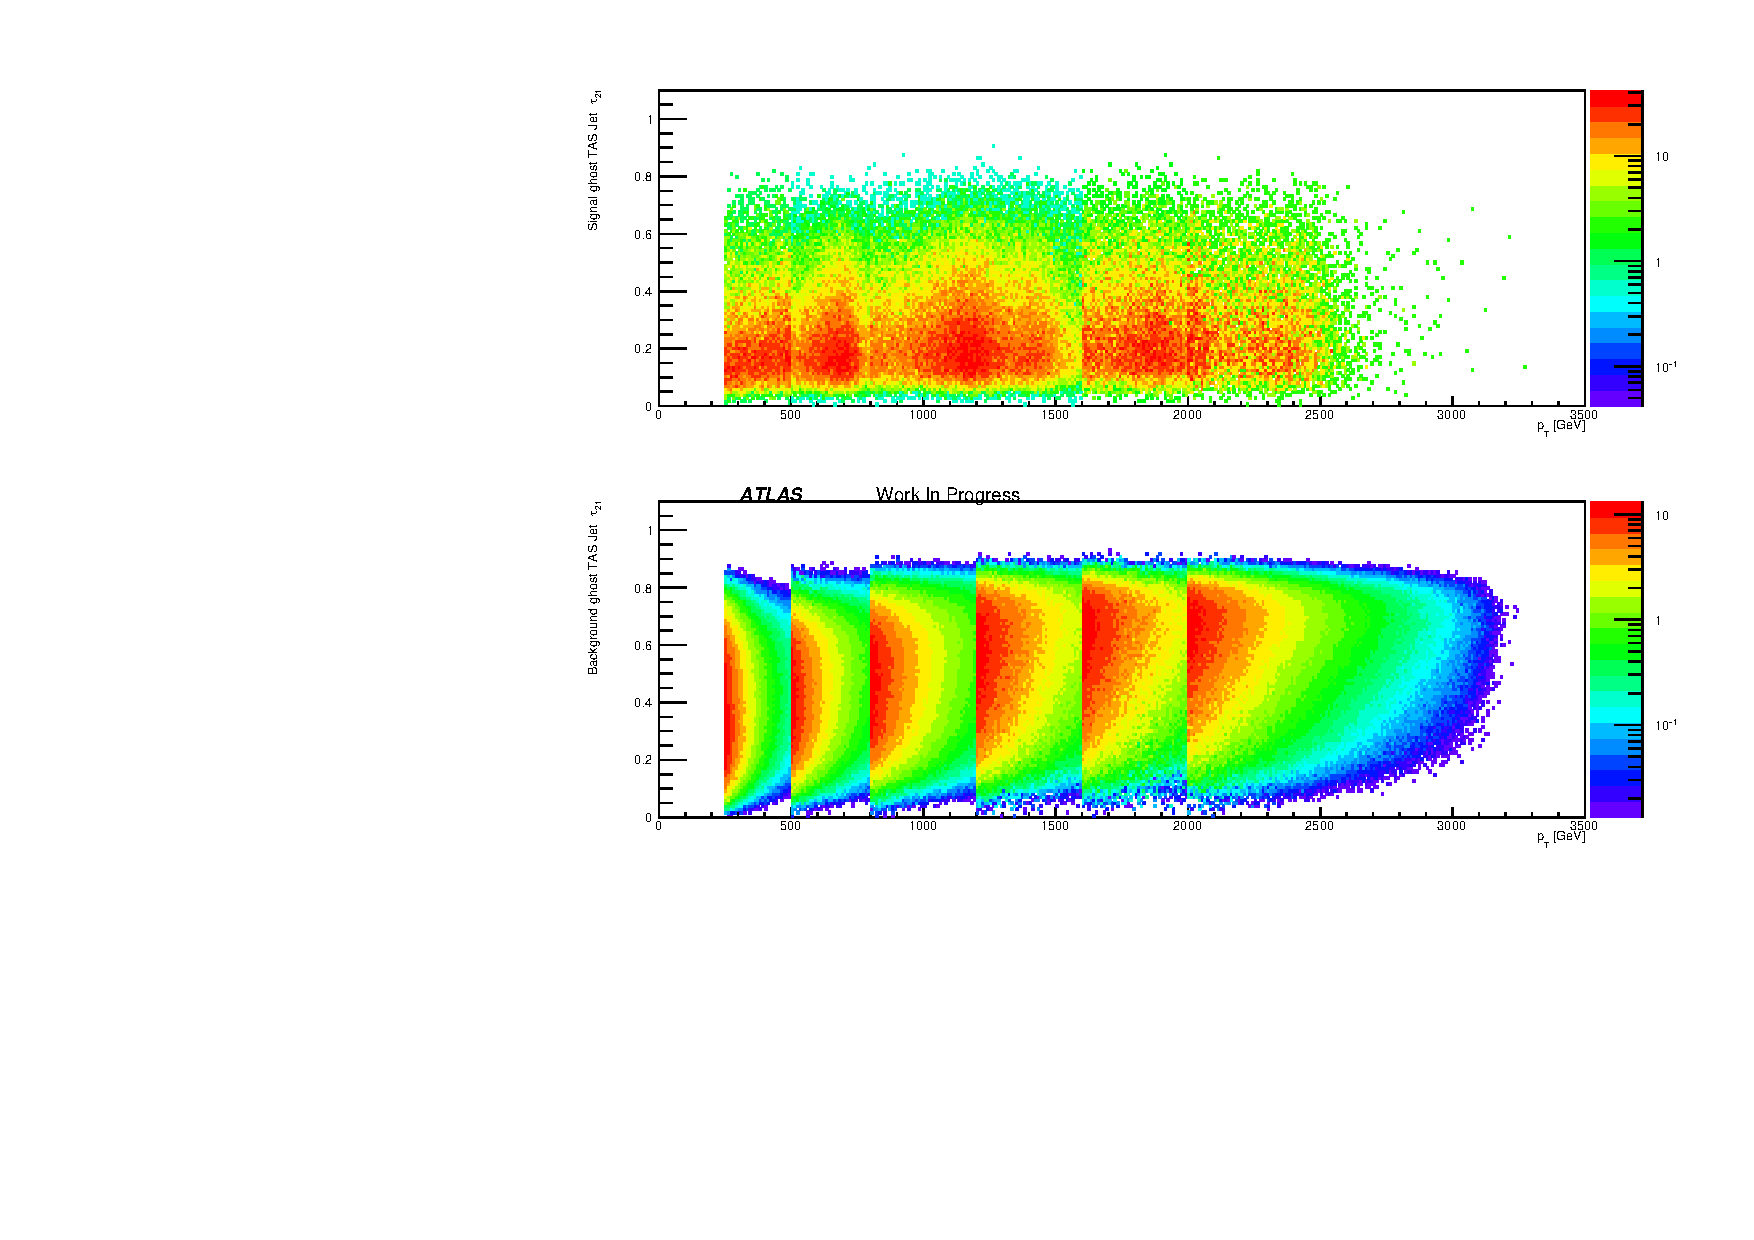
\includegraphics[width=0.5\textwidth]{sascha_input/plots/W/beta1/scatter_plots/scatter_h_scatter_assisted_tj_nSub21.pdf} 
\caption{\footnotesize{Correlation between $\tau_{21}$ at $\beta=1$ and $p_{\mathrm{T}}$ applied on $W$ boson signal (above) and QCD background (below) for calorimeter (left) and TAS (right).}}\label{fig:correlation_tau21}
\end{figure}

\subsubsection{Performance for Higgs boson tagging}\label{subsubsec:higgs_beta1}
The Higgs boson is heavier than the $W$ or $Z$ boson, resulting in a higher angular separation of the jet constituents considering the rule of thumb $\delta R \sim \frac{2m}{p_T}$ for decay products. As a result, angular resolution effects won't have the same impact as for the $W$ boson. This can be verified by the performance of track-based variables in the ROCs found in Figure \ref{fig:ROC_higgs_nSub21}.

For Higgs boson tagging and an angular weight of $\beta=1$, found were no distinct improvements with TAS or tracks compared to calorimeter clusters. The C2 variable performs better with calorimeter clusters, D2 yields an equal QCD discrimination with TAS and calorimeter clusters. The n-Subjettiness ratio $\tau_{21}$ benefits from TAS in some $p_{\mathrm{T}}$ regions, while the calorimeter pendant performs better in the other regions. Furthermore, tracks and TAS perform comparable over the whole studied $p_{\mathrm{T}}$ range. 
\begin{figure}[htp]
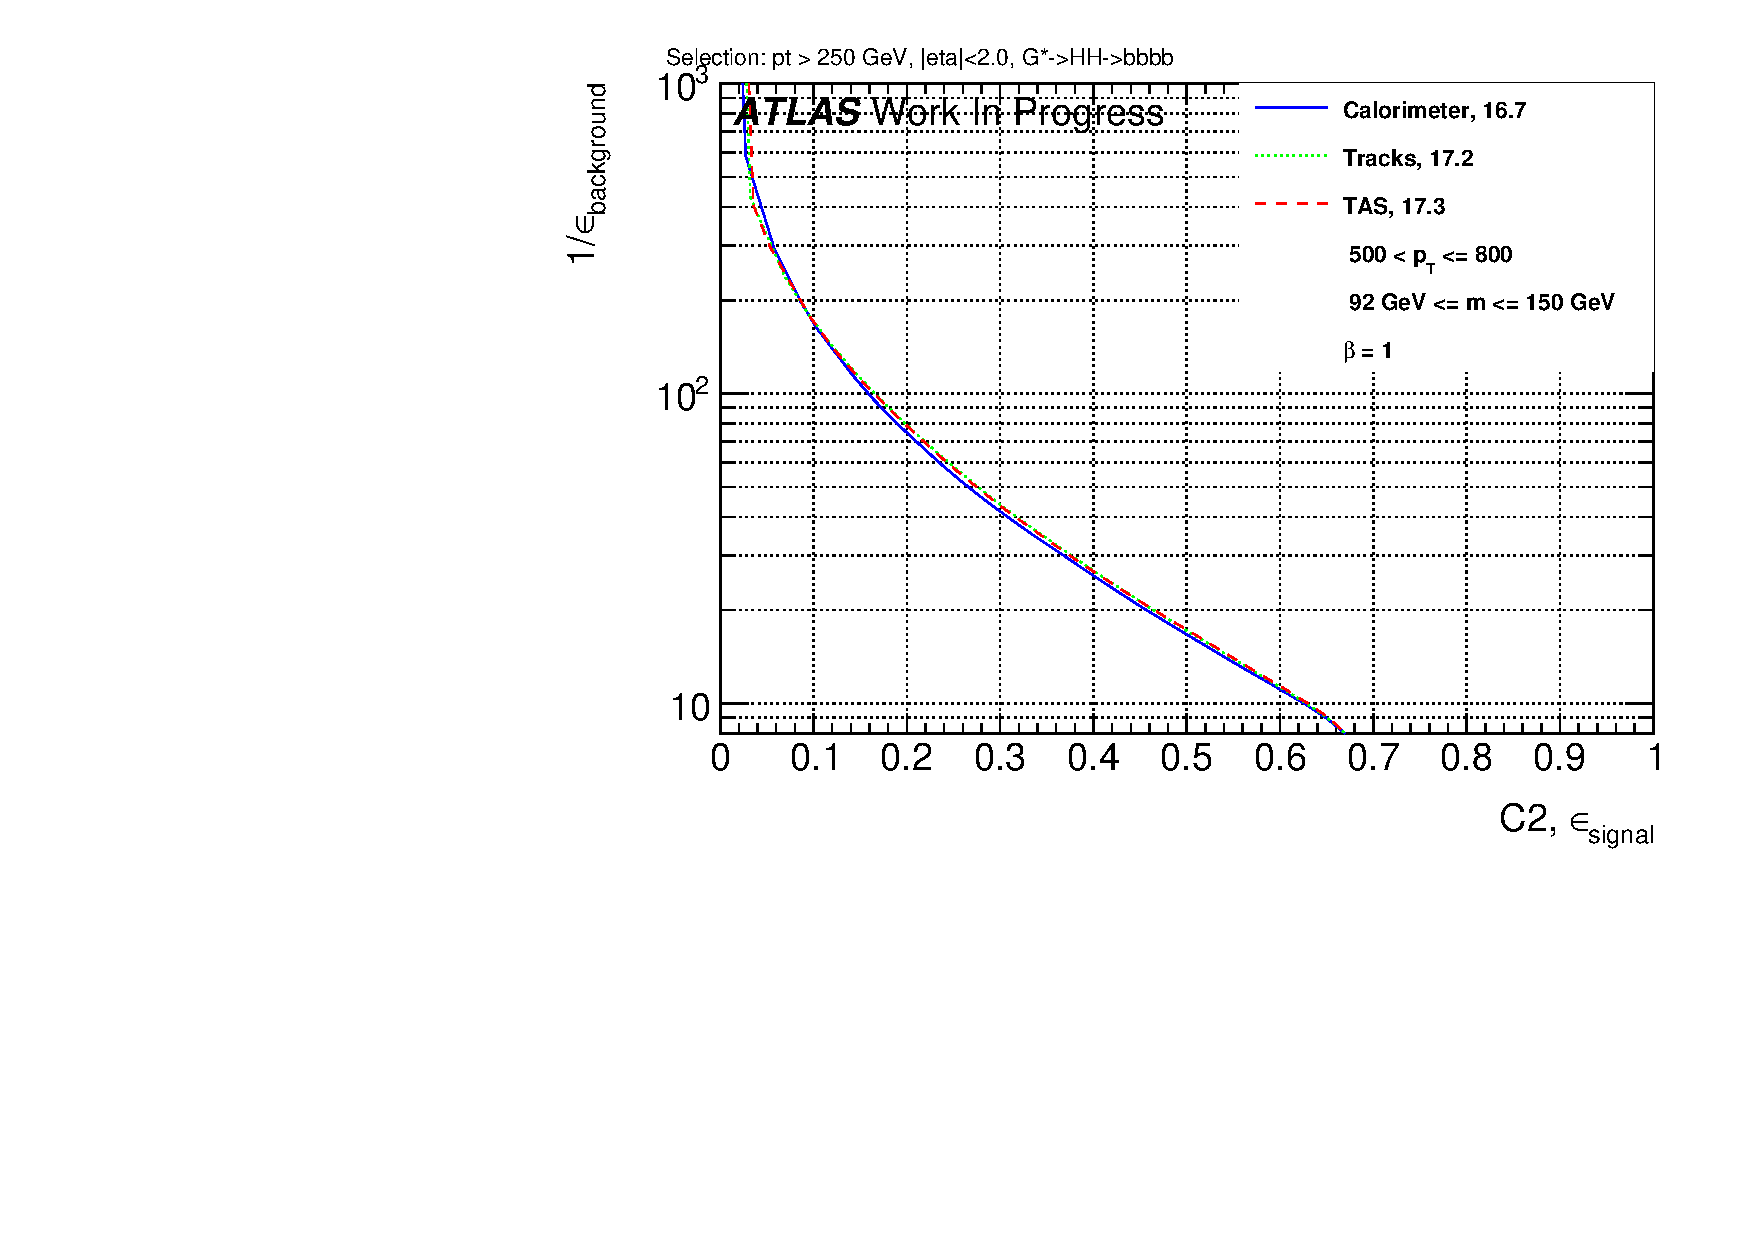
\includegraphics[width=0.3\textwidth]{sascha_input/plots/Higgs/ROC/Beta1/ROC_ALL_h_recoJet_C2_bin2.pdf} 
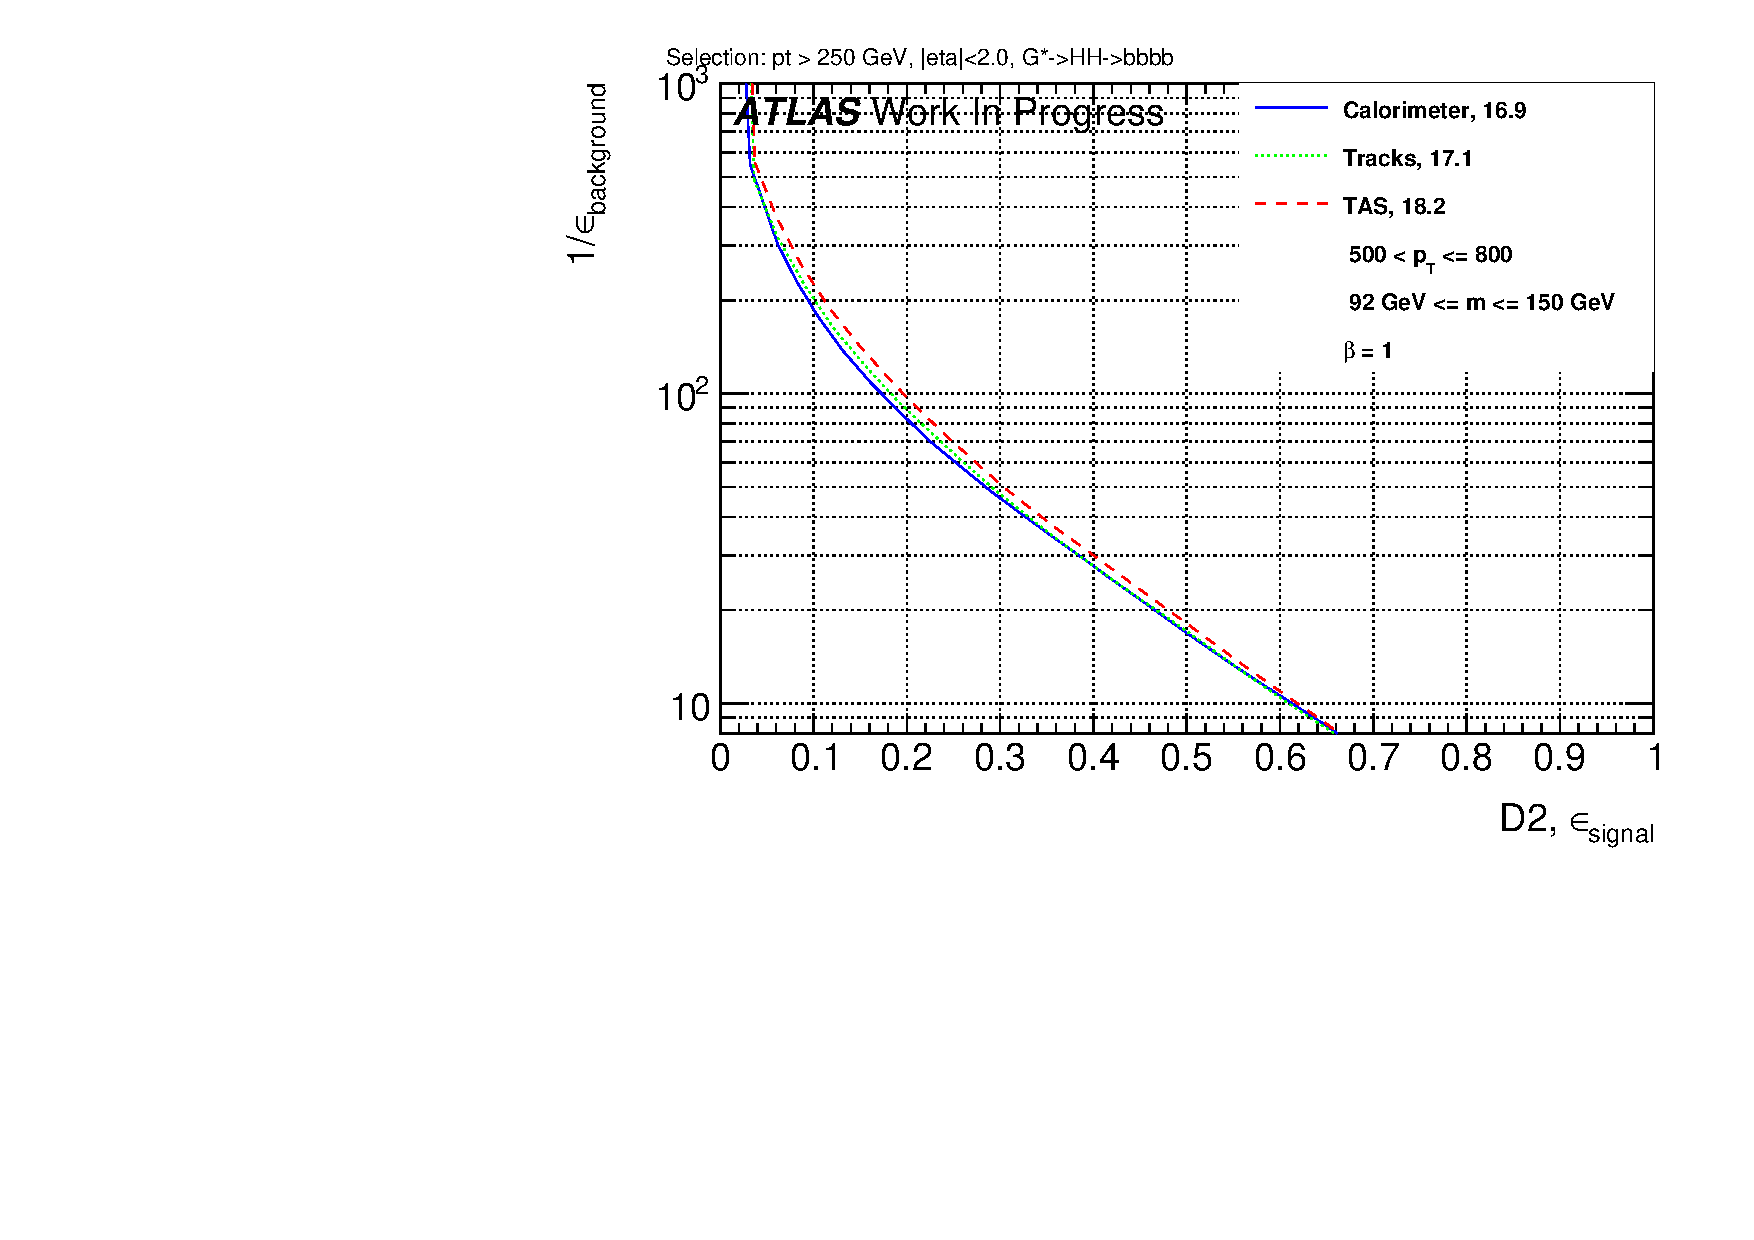
\includegraphics[width=0.3\textwidth]{sascha_input/plots/Higgs/ROC/Beta1/ROC_ALL_h_recoJet_D2_bin2.pdf} 
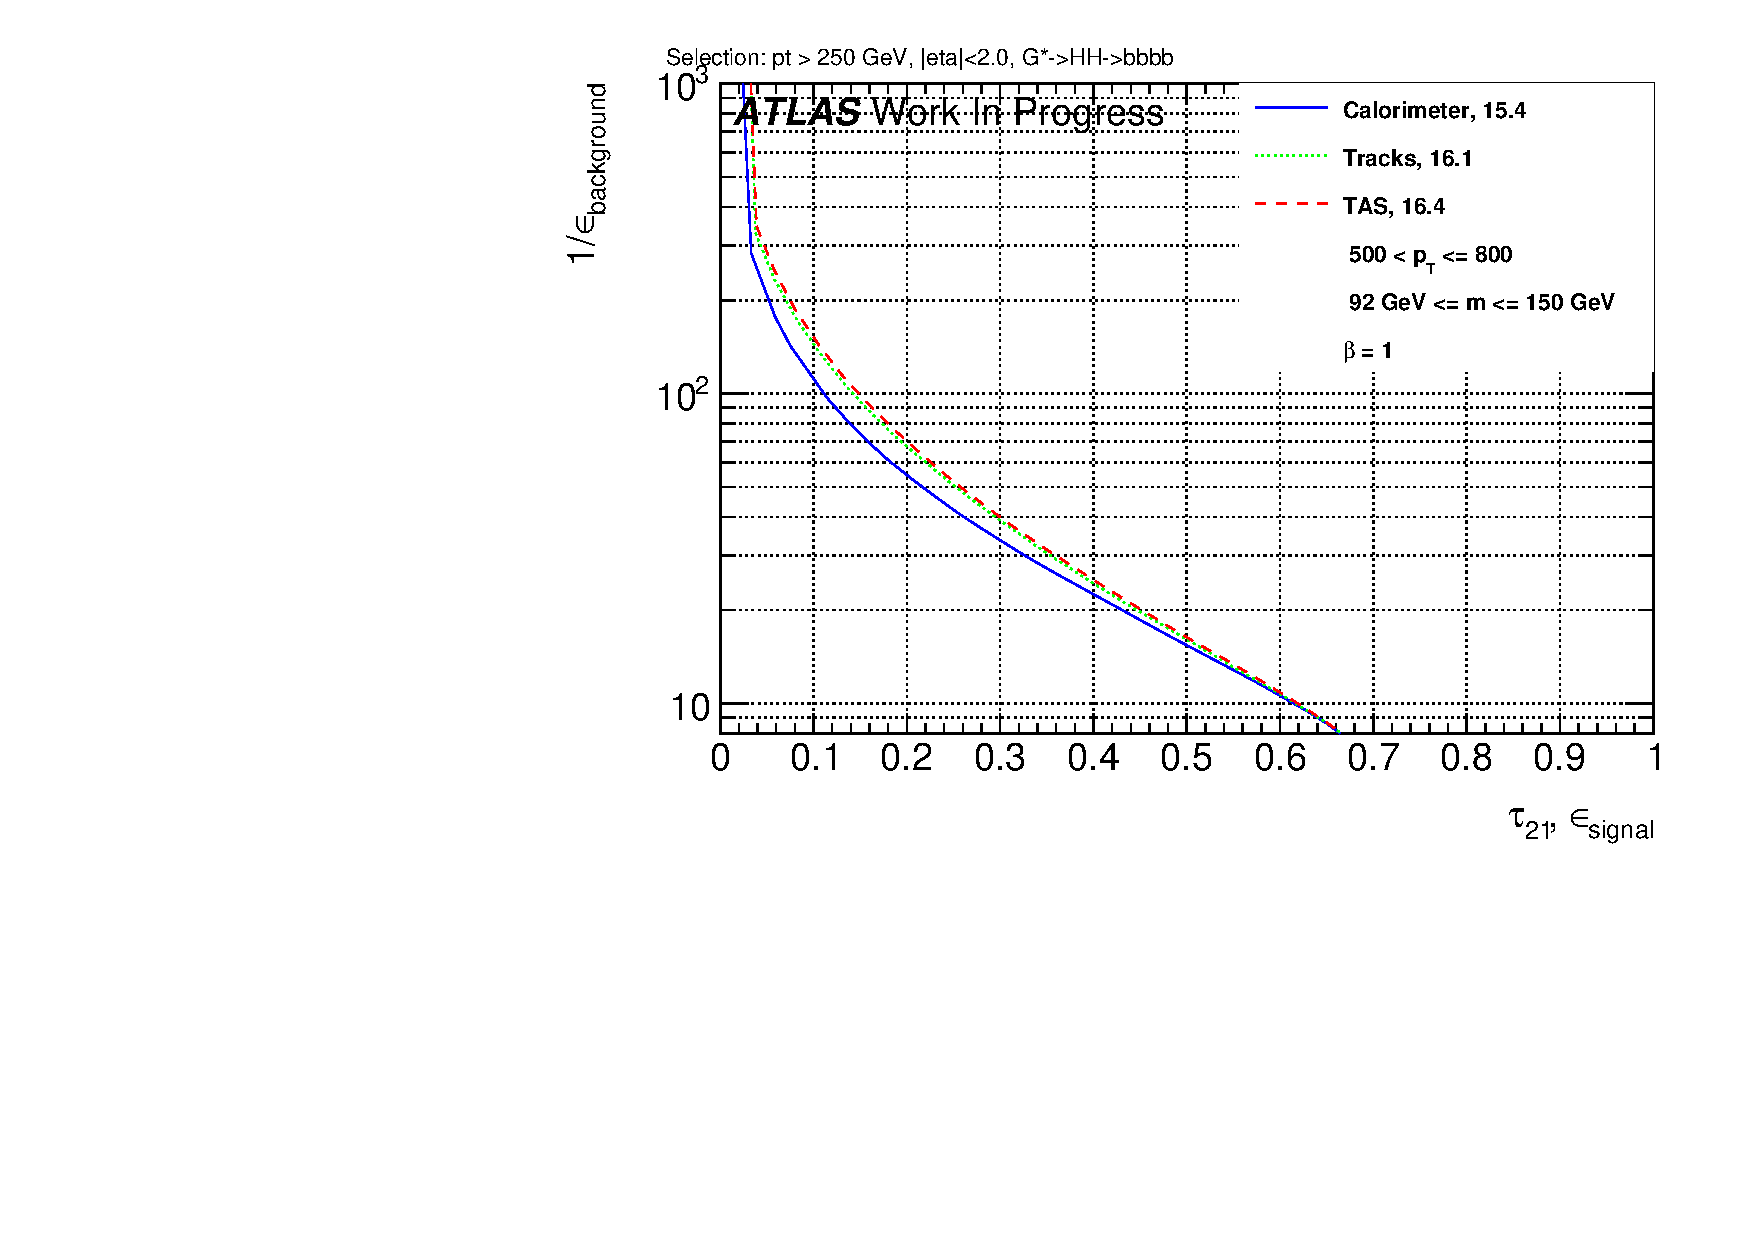
\includegraphics[width=0.3\textwidth]{sascha_input/plots/Higgs/ROC/Beta1/ROC_ALL_h_recoJet_nSub21_bin2.pdf}
\bigskip
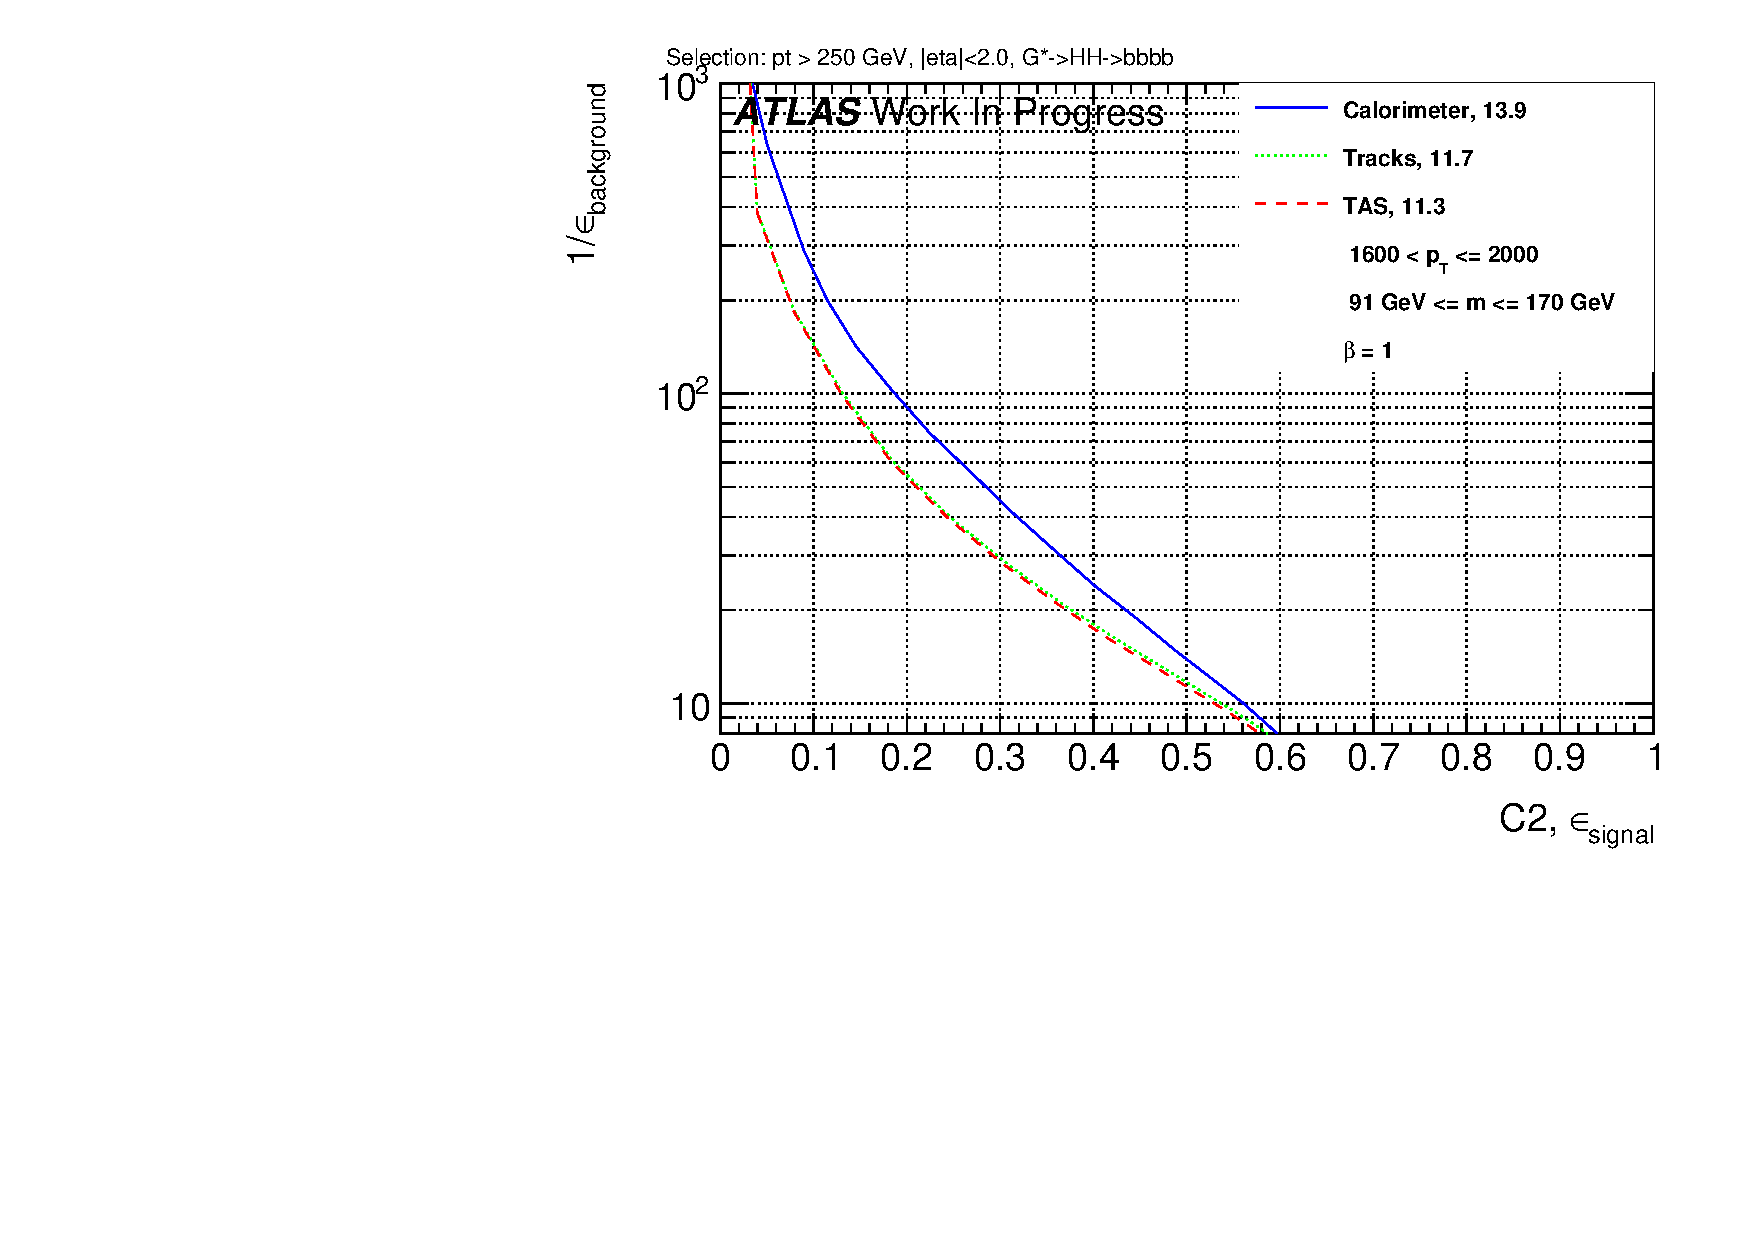
\includegraphics[width=0.3\textwidth]{sascha_input/plots/Higgs/ROC/Beta1/ROC_ALL_h_recoJet_C2_bin5.pdf} \hspace{6mm}
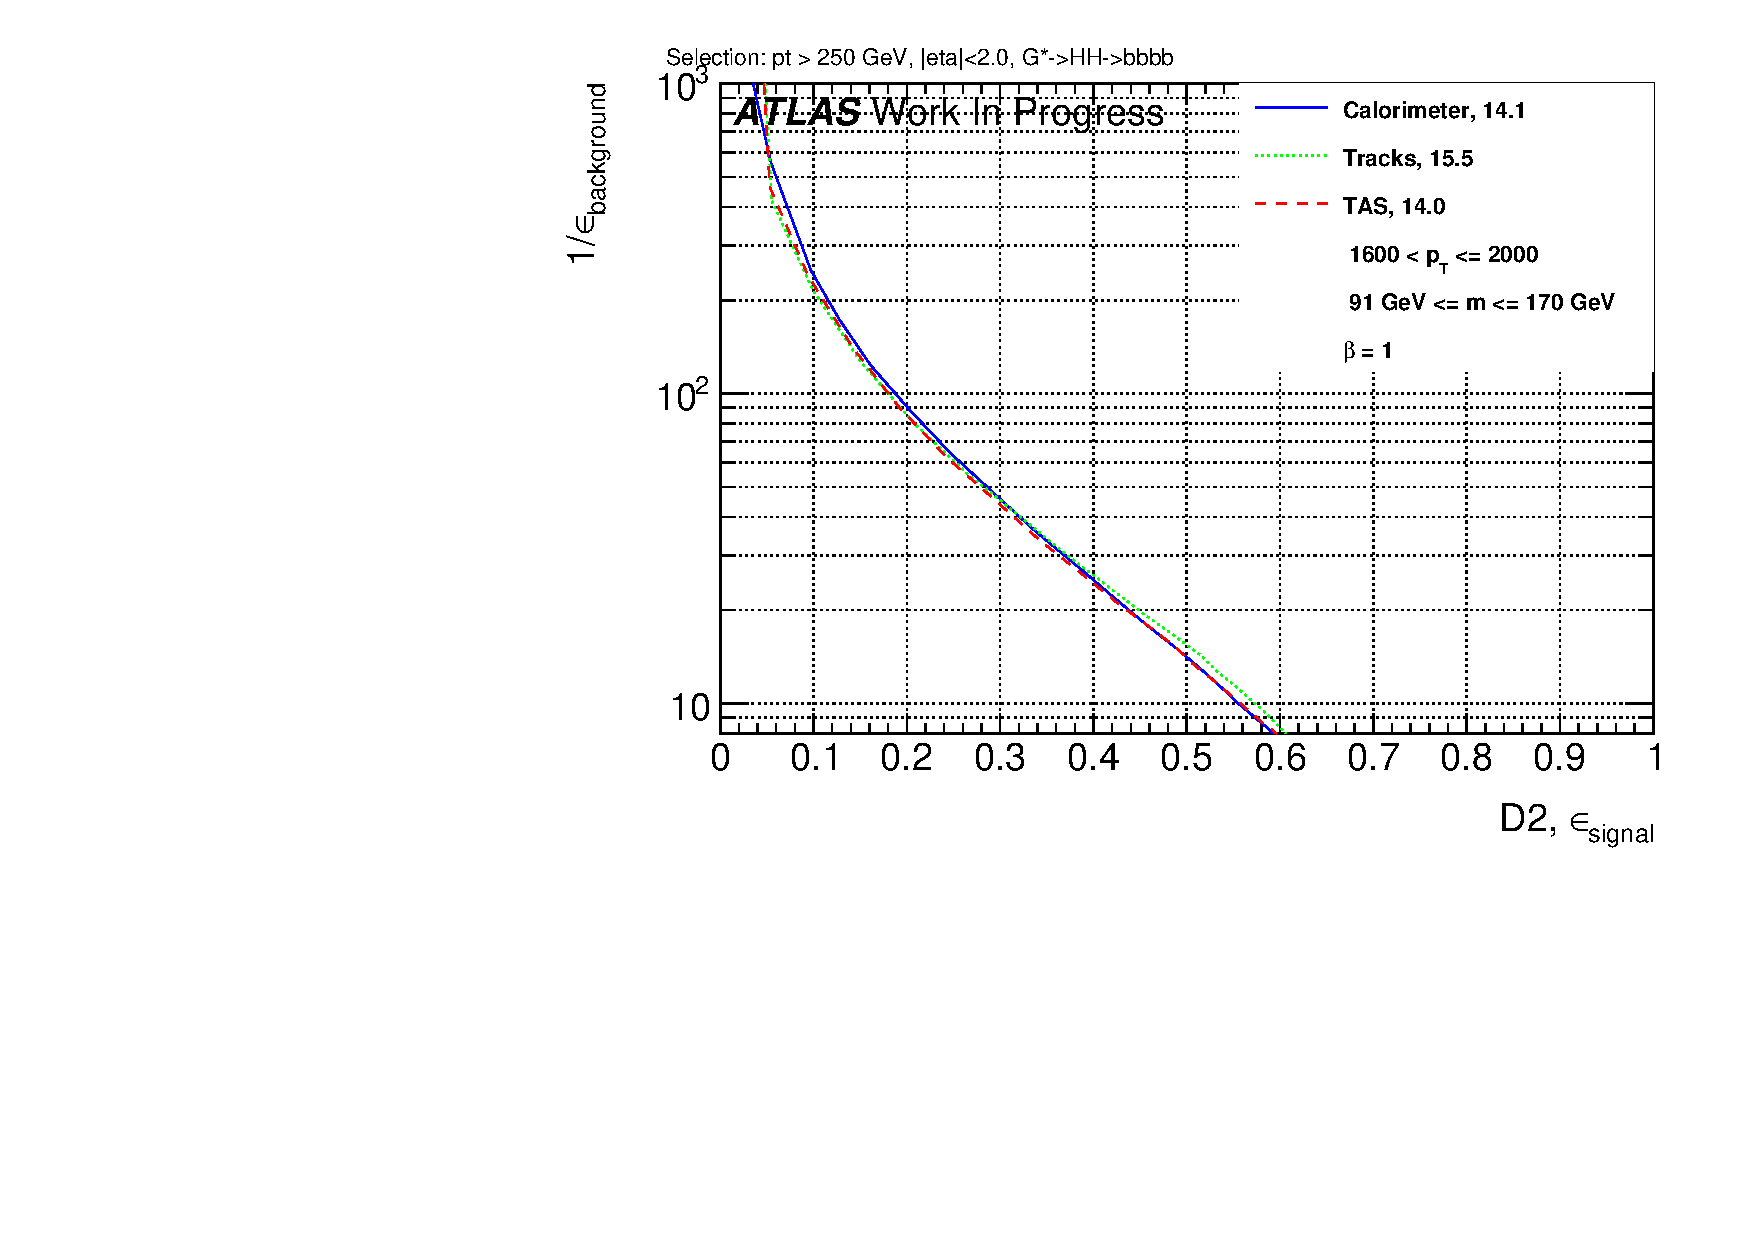
\includegraphics[width=0.3\textwidth]{sascha_input/plots/Higgs/ROC/Beta1/ROC_ALL_h_recoJet_D2_bin5.pdf} \hspace{6mm}
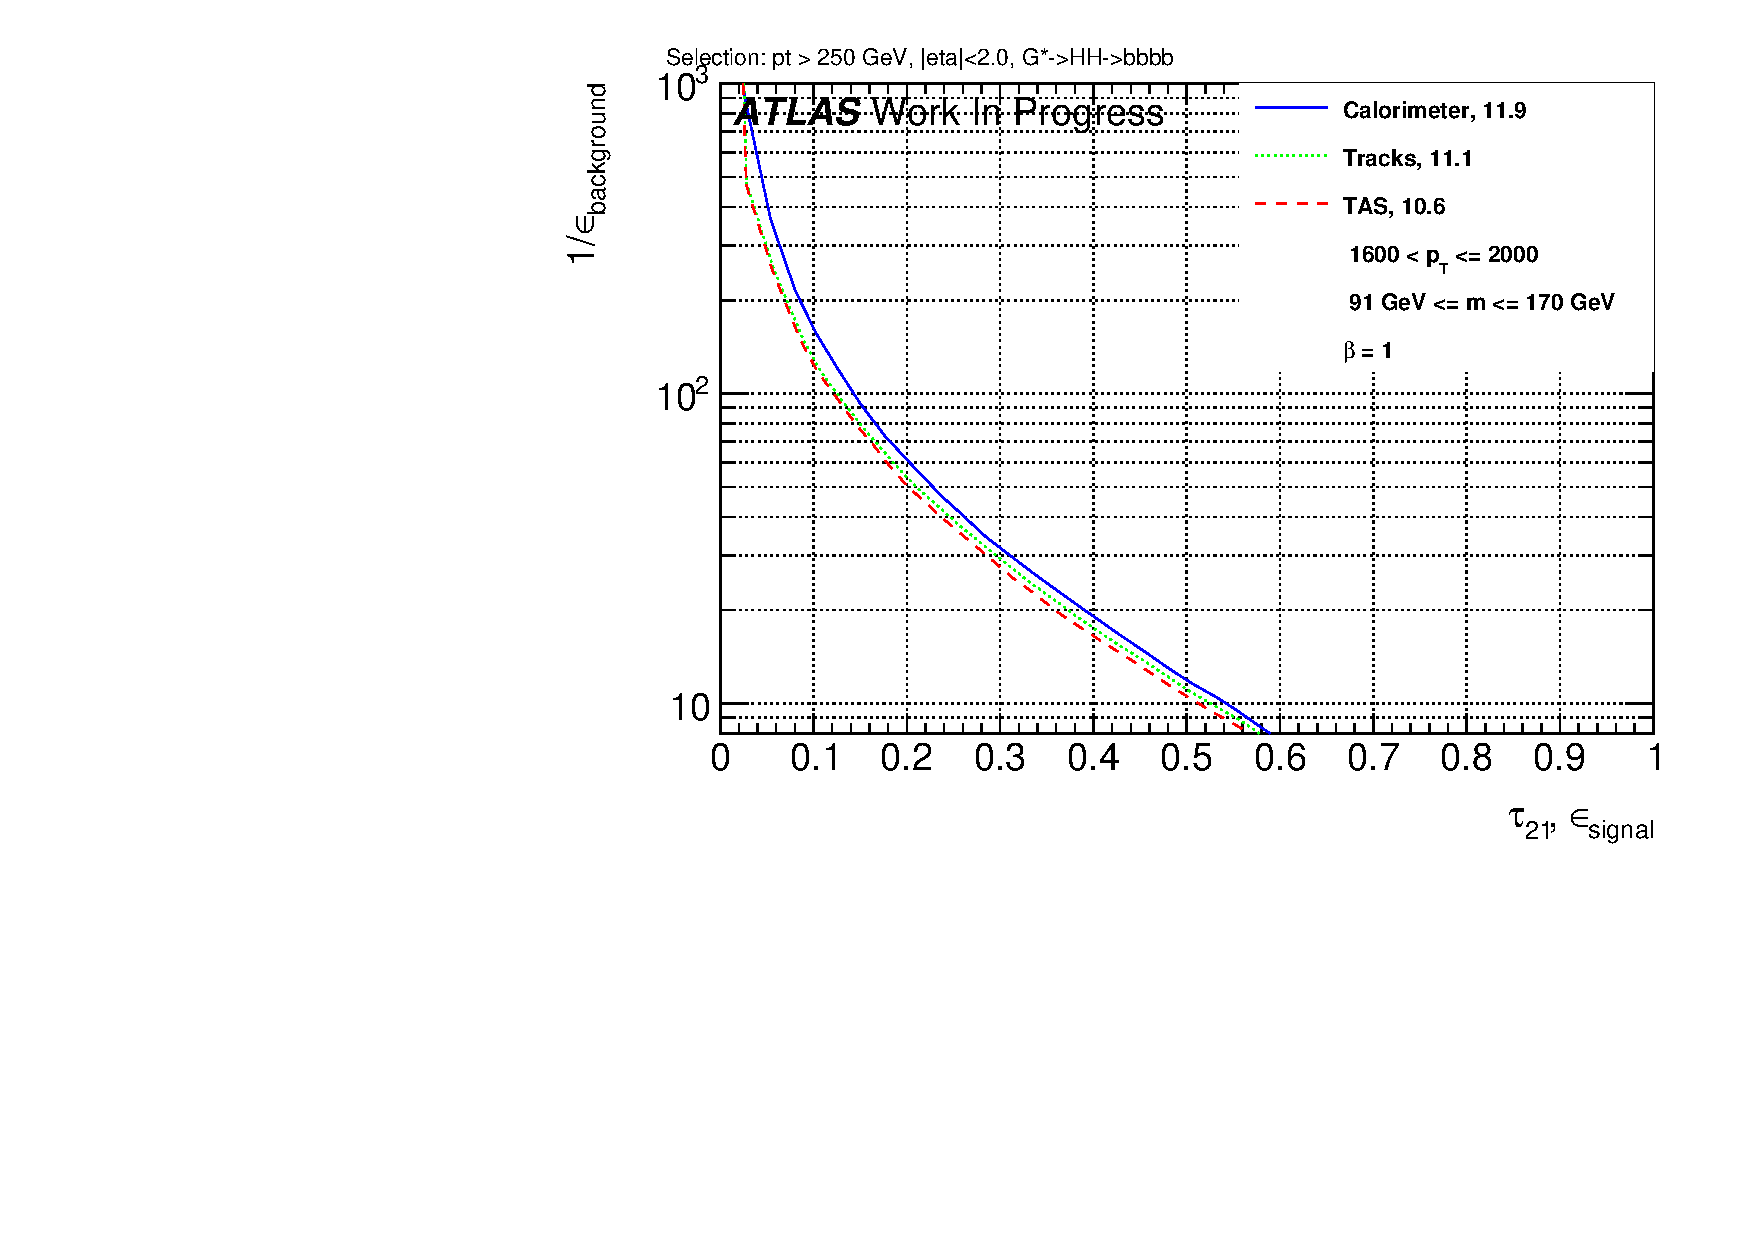
\includegraphics[width=0.3\textwidth]{sascha_input/plots/Higgs/ROC/Beta1/ROC_ALL_h_recoJet_nSub21_bin5.pdf}
\caption{\footnotesize{ROCs showing QCD rejection against Higgs boson efficiency for tracks, TAS and colorimeter. C2 (left), D2 (middle) and $\tau_{21}$ (right) at $\beta=1$. Shown is the energy range between 500-800 GeV (top) and 1600-2000 GeV (bottom). The numbers in the legend second $p_{\mathrm{T}}$ bin (left) and highest bin (right). The numbers in the legend indicate the achieved background rejection at 50\% signal efficiency.}}\label{fig:ROC_higgs_nSub21}
\end{figure}

\subsubsection{Performance for Top quark tagging}
The top quark features a characteristic three body decay and a very high mass around $173 \, \text{GeV}$. Studied here is the n-Subjettiness ratio $\tau_{32}$ to distinguish the three prong like top quark jets and QCD background jets.

The ROCs in Figure \ref{fig:ROC_top} show the accompanying improvements in the separation power of $\tau_{32}$ possible with TAS. Tagging tops quark events with $\tau_{32}$ is found to greatly benefit from the excellent angular resolution of tracks. This is especially the case for high $p_{\mathrm{T}}$ where the limitation of the calorimeter cell size clearly diminishes the possible identification of three distinct substructures inside a large-R jet. The enhancements are not as articulated for the low $p_{\mathrm{T}}$ regions, nevertheless TAS $\tau_{32}$ performs here at least equally well as calorimeter $\tau_{32}$. Furthermore, tracks are observed to perform slightly worse in comparison with TAS for the lower $p_{\mathrm{T}}$ regions, but match the TAS performance for very large boosts as expected.
\begin{figure}[htp]
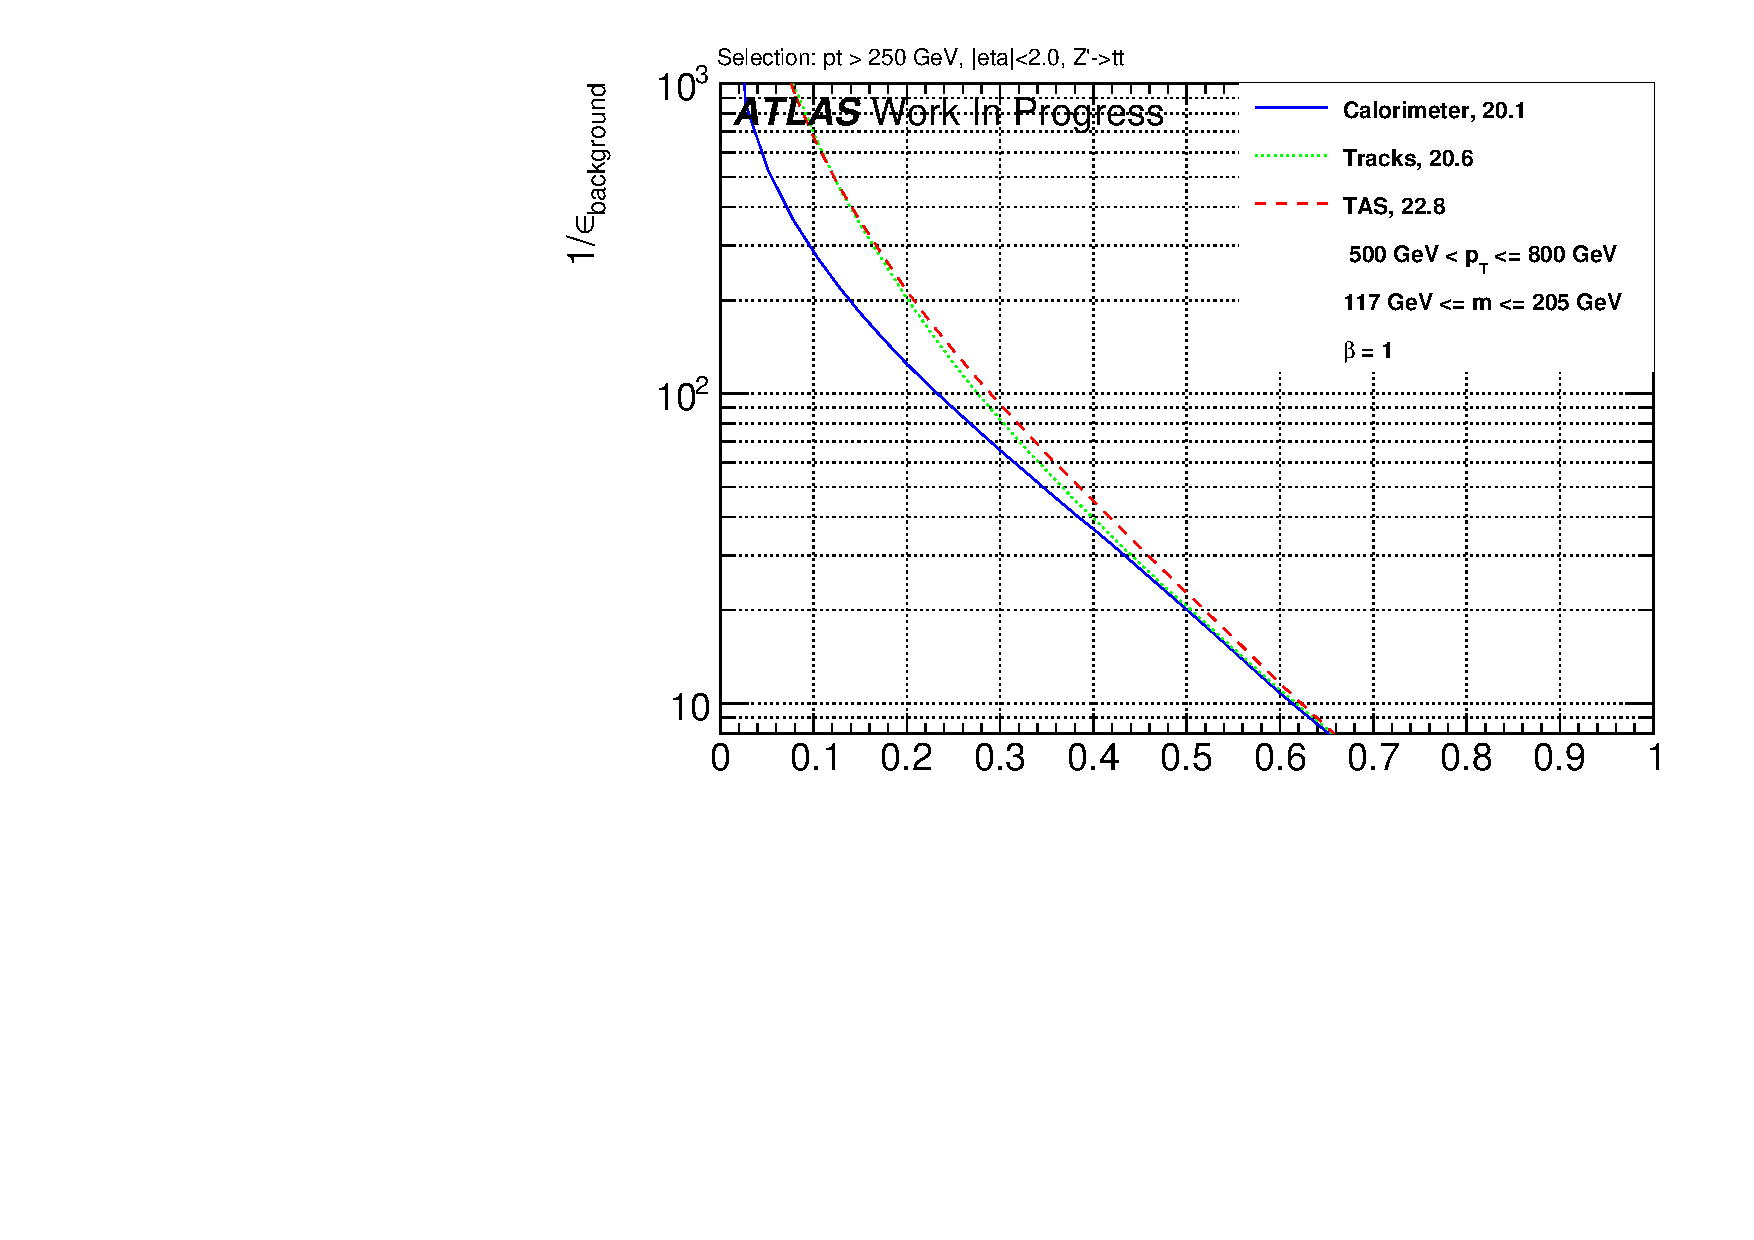
\includegraphics[width=0.5\textwidth]{sascha_input/plots/Top/beta1/ROC_ALL_h_recoJet_nSub32_bin2.pdf} \hspace{1mm}
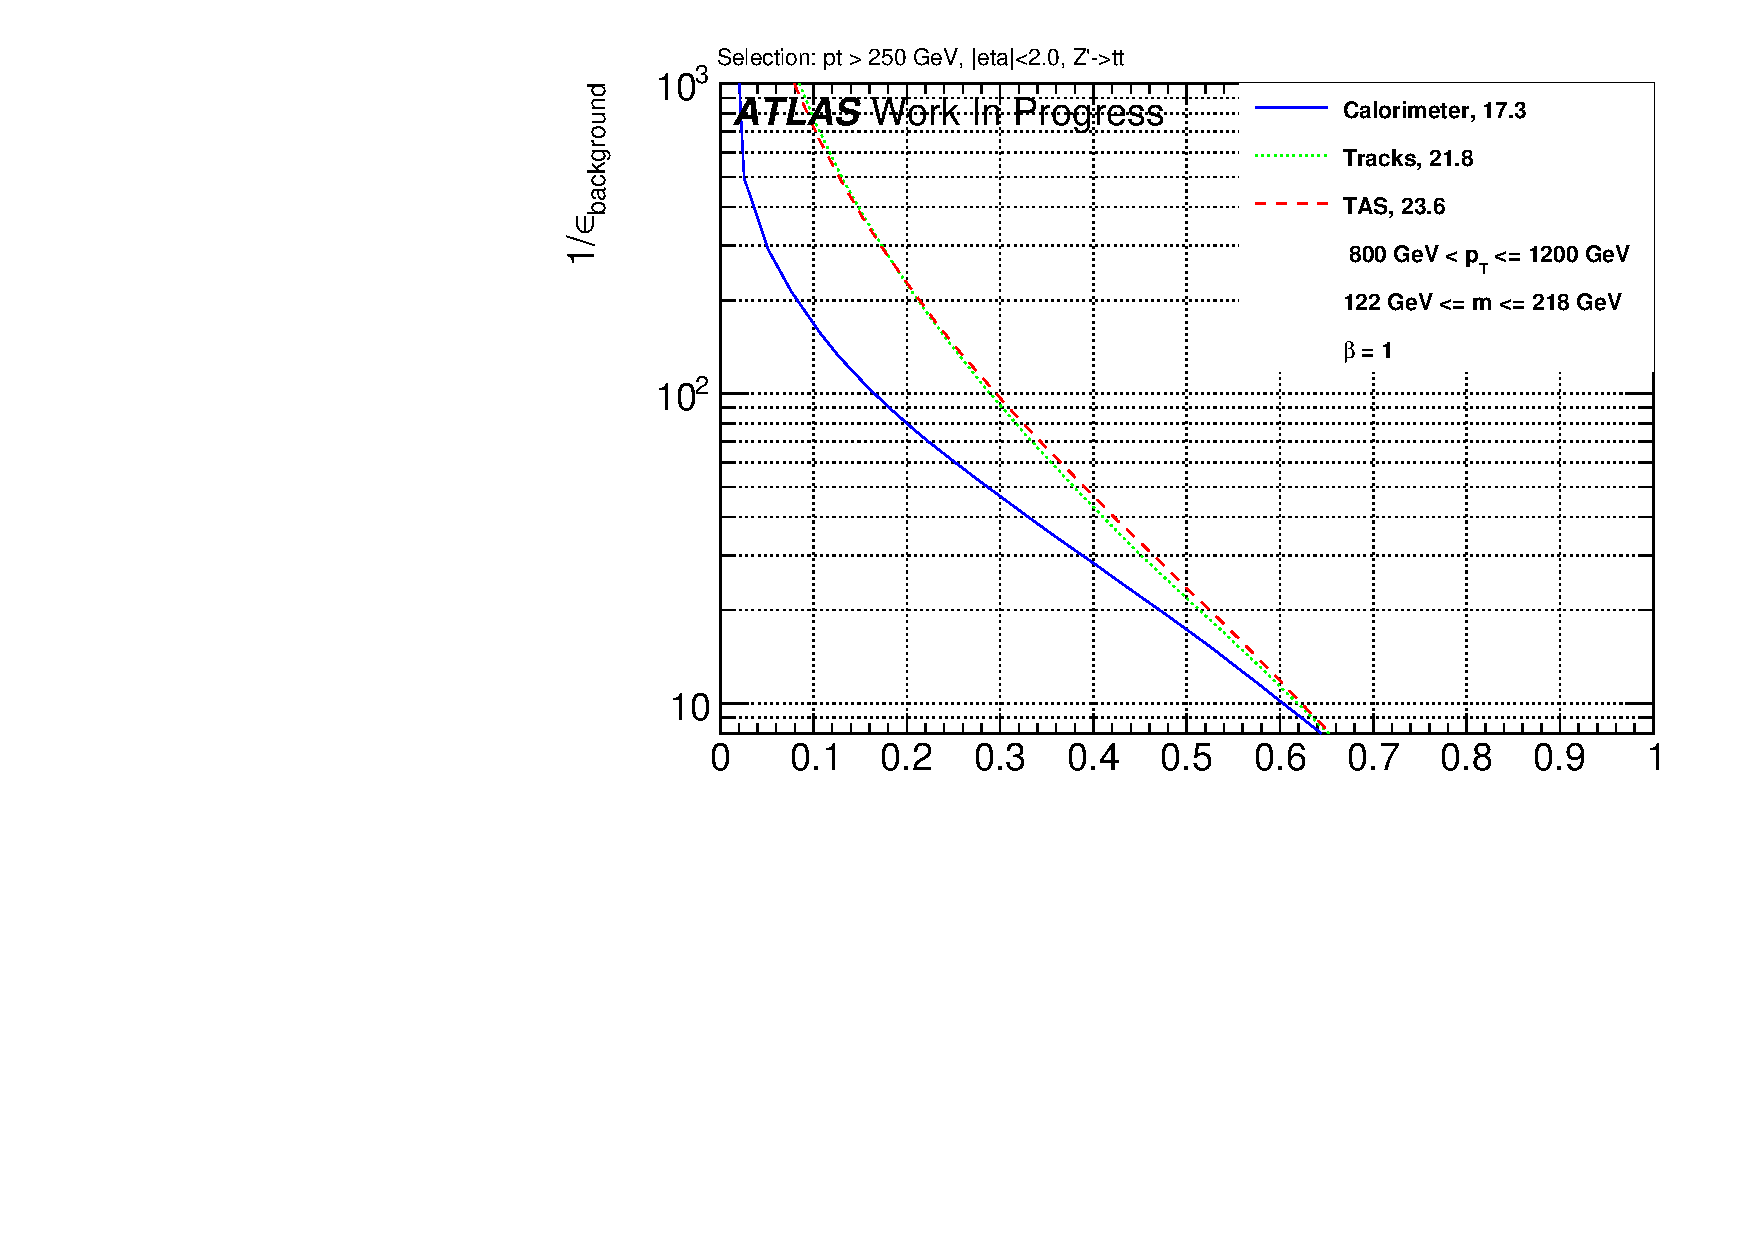
\includegraphics[width=0.5\textwidth]{sascha_input/plots/Top/beta1/ROC_ALL_h_recoJet_nSub32_bin3.pdf}
\bigskip
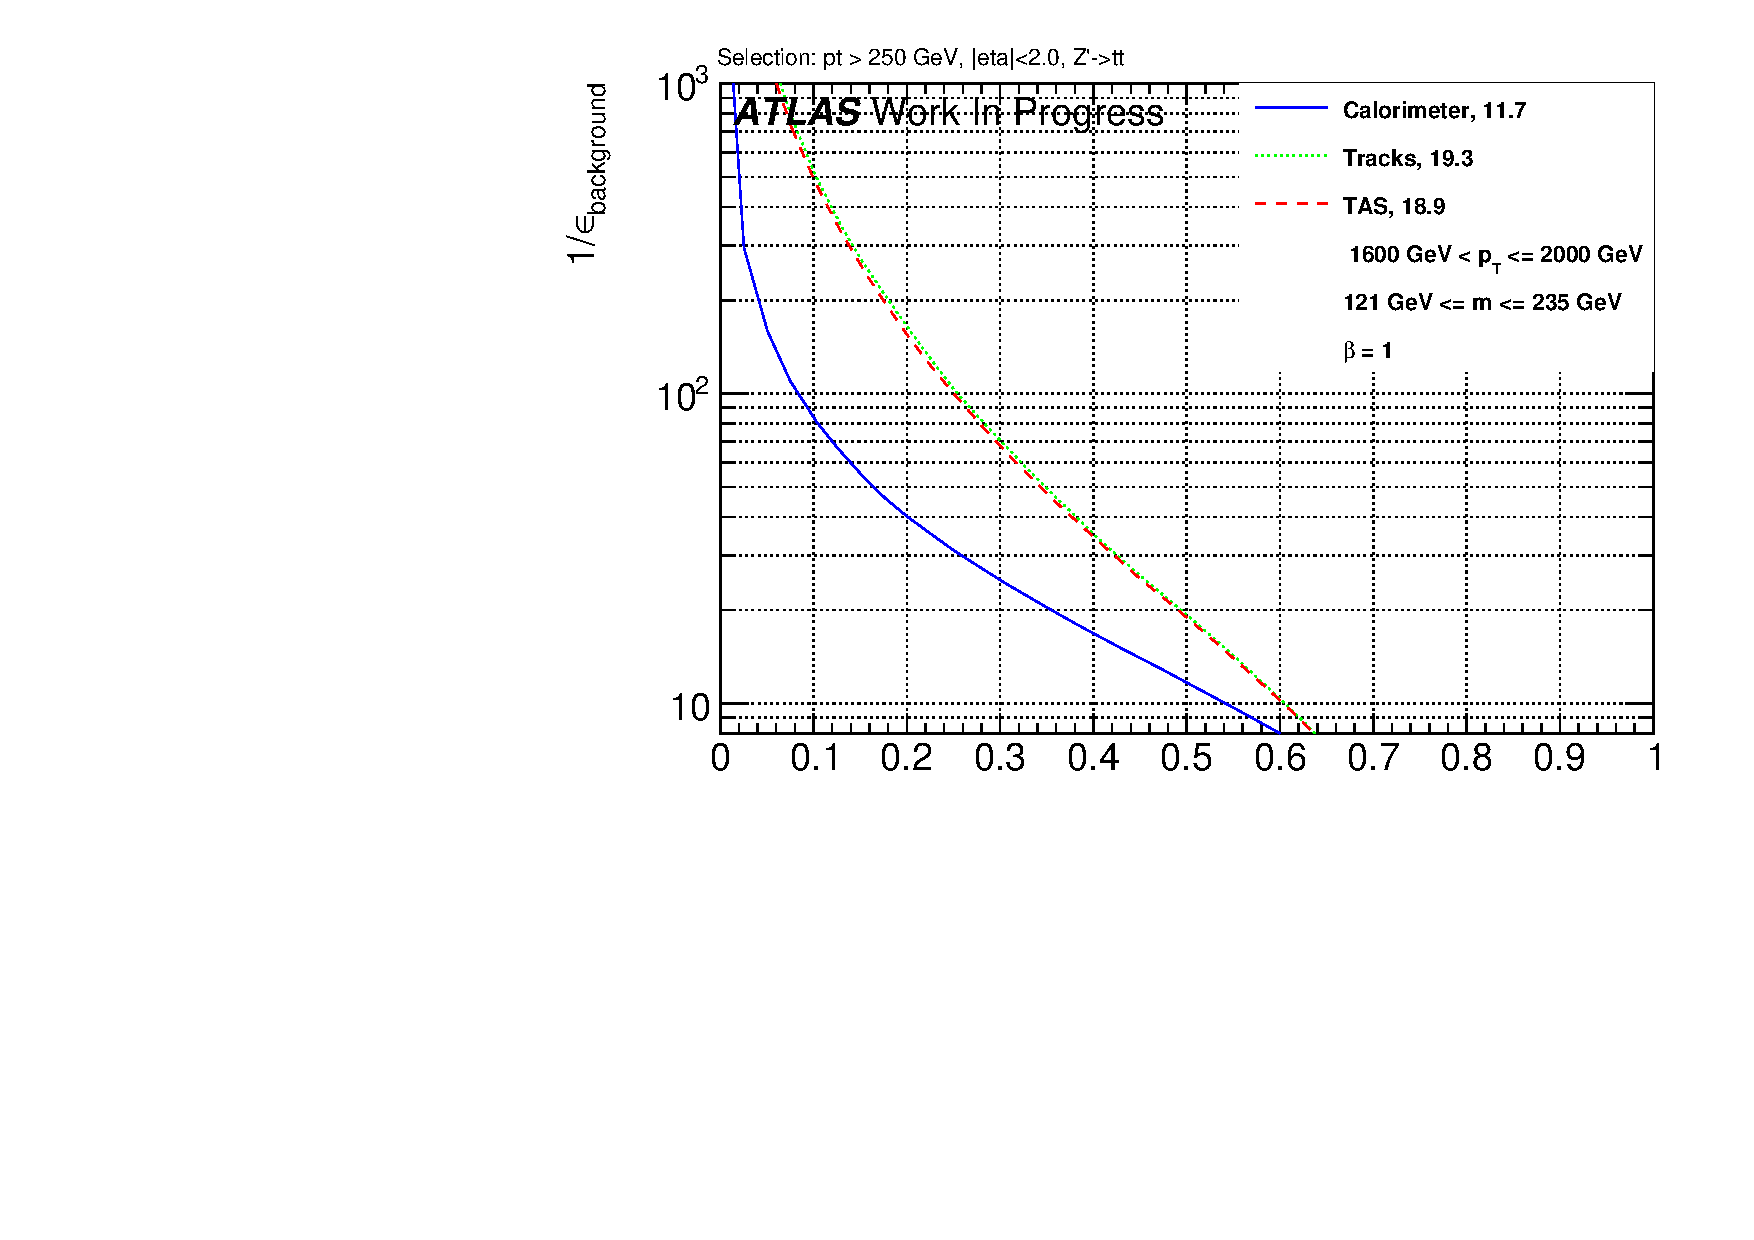
\includegraphics[width=0.5\textwidth]{sascha_input/plots/Top/beta1/ROC_ALL_h_recoJet_nSub32_bin5.pdf} \hspace{1mm}
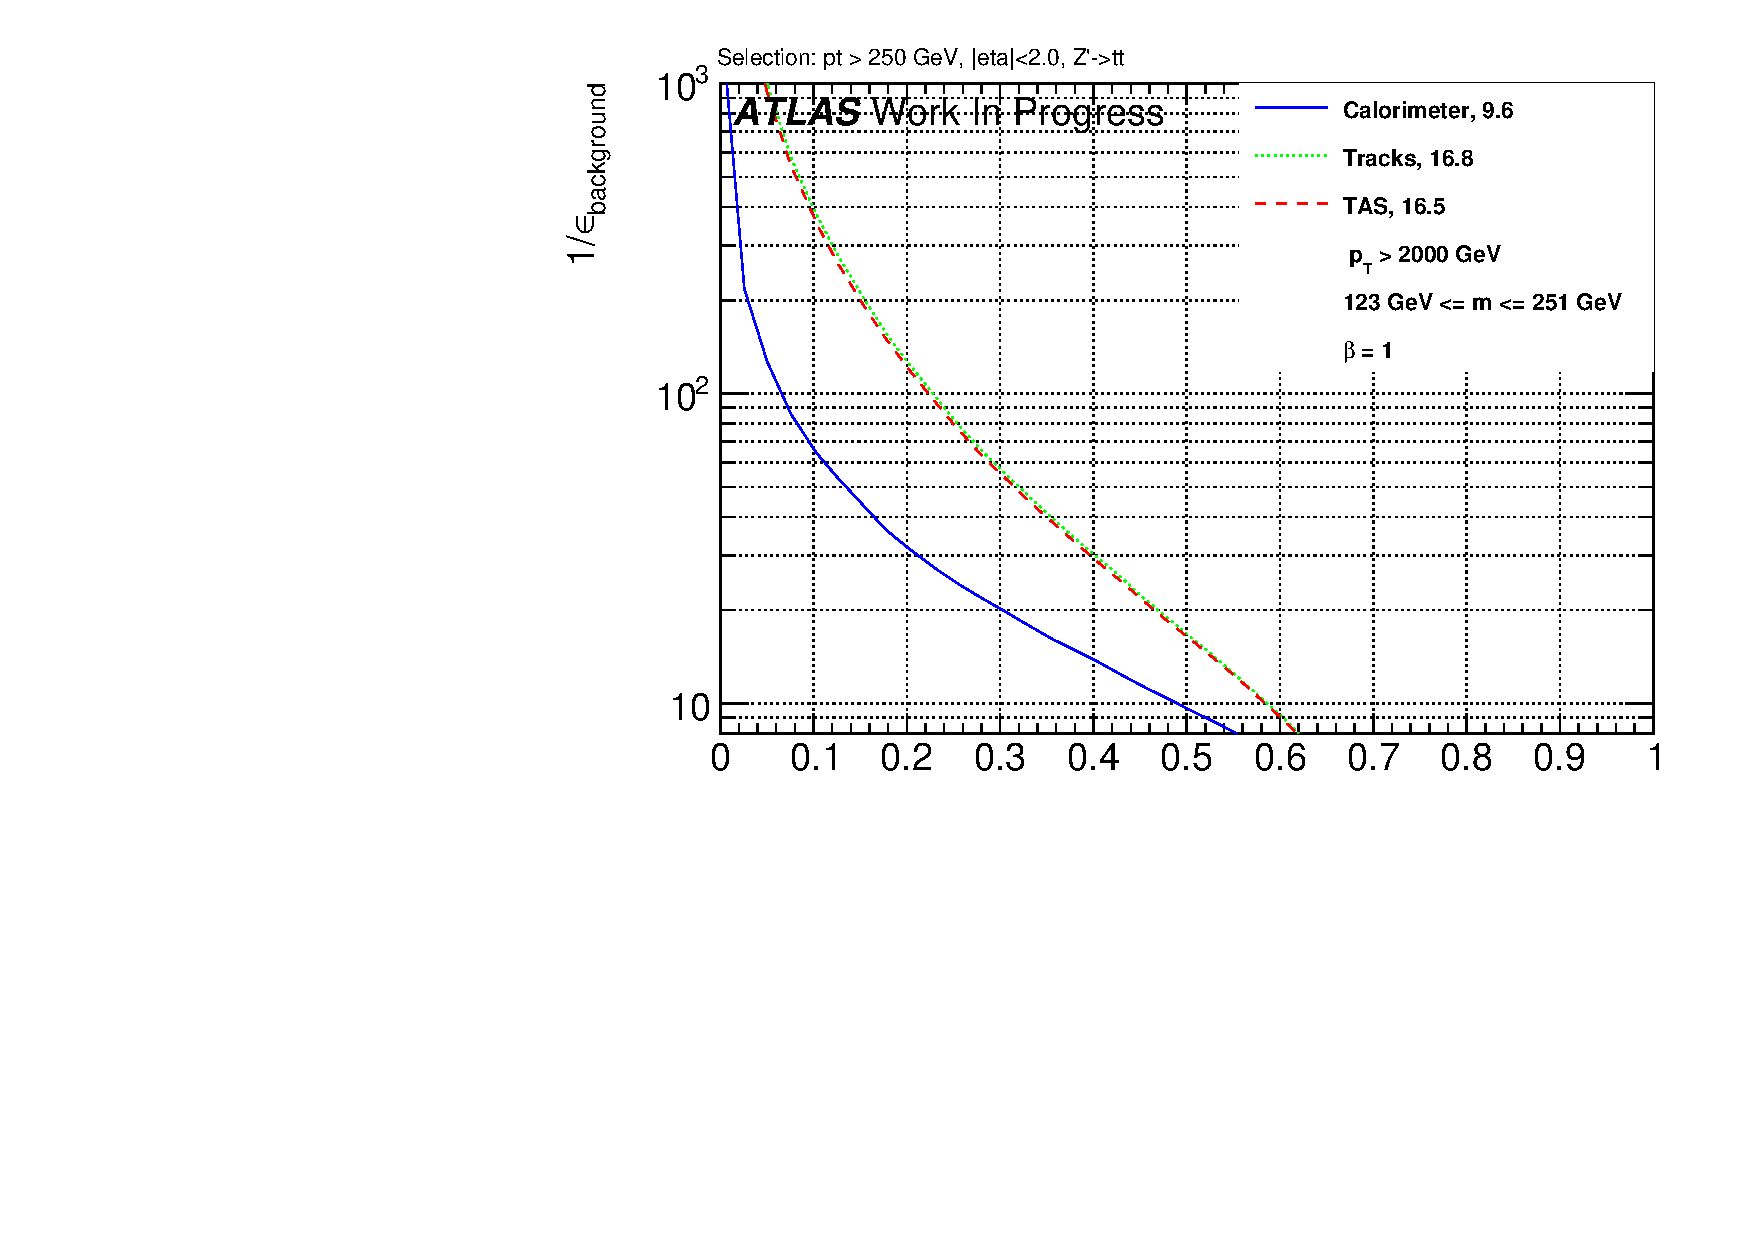
\includegraphics[width=0.5\textwidth]{sascha_input/plots/Top/beta1/ROC_ALL_h_recoJet_nSub32_bin6.pdf}
\caption{\footnotesize{ROCs showing QCD rejection against top quark efficiency for tracks, TAS and colorimeter $\tau_{32}$ at $\beta=1$, $p_{\mathrm{T}}$ ordering from upper left to lower right.}}\label{fig:ROC_top}
\end{figure}



